\chapter{Motivation \& Tools from the Continuum}
\label{chap:background}

In this chapter, I lay out the physics context of this work and some theoretical machinery that was useful for this work. This section consists of a definition and the empirical status of the Standard Model. Then, I will expand on the details of the specific sector we are interested in - the flavor sector and the CKM matrix.

I will also summarize some physics machinery useful for this work, namely QCD, chiral symmetry, and effective field theories for heavy quarks.

\section{Testing the Standard Model}

The Standard Model of Particle Physics (SM) \cite{GLASHOW1961579,PhysRevLett.19.1264,Salam:1968rm} is, so far, the most successful theory for describing fundamental particles and their interactions. It is an effective Yang-Mills quantum field theory. It is most succinctly defined by listing its symmetries, field content, and the irreducible representations (irreps) of the symmetries that those fields transform under. Below I follow the discussion in \cite{Schwartz:2013pla}.

The symmetries are the following. The Lorentz group $SO(3,1)$, the group of coordinate transformations that leave the Minkowski metric invariant, which can be decomposed into $SU(2)_l\times SU(2)_r$ ({\it{left-handed}} and {\it{right-handed}}). We denote an irrep as $(a,b)$ where $a$ is the $\sigma^z$ eigenvalue under $SU(2)_l$ transforms, and $b$ is that of $SU(2)_r$. Then there are internal local gauge symmetries:
\begin{align}
  SU(3)_C\times SU(2)_L \times U(1)_Y,
\end{align}
irreps of which we denote with $(x,y,z)$, where $x,y$ label the $SU(3)_C$ and $SU(2)_L$ irreps and $z$ is the charge under $U(1)_Y$. The subscript $C$ stands for color, $L$ stands for 

The field content is: gauge bosons for each of the above gauge symmetries, each transforming in the adjoint of their corresponding symmetry and in the $(1/2,1/2)$ irrep of the Lorentz group, denoted $B_{\mu}$, $W_{\mu}$, $G_{\mu}$ respectively. There are 6 $SU(2)_L$ doublets in the $(1/2,0)$ Lorentz irrep; the {\it{left-handed fermions}}:
\begin{align}
  Q_{1,2,3} =&
  \begin{pmatrix} u_L \\ d_L \end{pmatrix},
  \begin{pmatrix} c_L \\ s_L \end{pmatrix},
  \begin{pmatrix} t_L \\ b_L \end{pmatrix}
  ,\quad\quad
  (\mathbf{3},\mathbf{2},1/6) \\
  L_{1,2,3} =&
  \begin{pmatrix} \nu_{e,L} \\ e_L \end{pmatrix},
  \begin{pmatrix} \nu_{\mu,L} \\ \mu_L \end{pmatrix},
  \begin{pmatrix} \nu_{\tau,L} \\ \tau_L \end{pmatrix}
  ,\quad\quad
  (\mathbf{1},\mathbf{2},-1)
\end{align}
and 9 $SU(2)_L$ singlets in the $(0,1/2)$ Lorentz irrep; the {\it{right-handed fermions}}:
\begin{align}
  u^R_{1,2,3} &= u_R, c_R, t_R\,,\quad\quad (\bar{\mathbf{3}},\mathbf{1},2/3) \\
  d^R_{1,2,3} &= d_R, s_R, b_R\,,\quad\quad (\bar{\mathbf{3}},\mathbf{1},-1/3) \\
  e^R_{1,2,3} &= e_R, \mu_R, \tau_R\,,\quad\quad (\mathbf{1},\mathbf{1},-1).
\end{align}
We have also listed the SM gauge irreps next to each definition. There is also in principle a further set of right-handed $SU(2)_L$ singlets, $\nu^R_{1,2,3} = (\nu_{e,R}, \nu_{\mu,R}, \nu_{\tau,R})$, but these are singlets of the entire SM gauge group so in a phenomenological sense are very much `not there'. There is also a Lorentz scalar $SU(2)_L$ doublet, the Higgs $H$, in gauge irrep $({\bf{1}},{\bf{2}},1/2)$ \cite{PhysRevLett.13.321,PhysRevLett.13.508,PhysRevLett.13.585}. $H$ obtains a vacuum expectation value under $\sim 200$GeV and causes a breaking of the above gauge group to $SU(3)_C\times U(1)_E$, where $U(1)_E$ is the electromagnetic gauge group mediated by the photon.
\\ \\
There is at present no confirmed evidence of physics beyond the SM (or {\it{new physics}}), besides the presence of neutrino ($\nu$) masses \cite{GONZALEZGARCIA20081}. However, there are a number of problems with the SM that heavily imply that there must be new physics. Among the most famous sources of concern are:
\begin{itemize}
\item
  {\bf{Dark Matter \& Dark Energy}} - an estimated 96\% of the content of the universe is dark matter \cite{Freese:2008cz} and dark energy \cite{Riess:1998cb,Perlmutter:1998np}, that does not interact with the SM gauge group (only via gravity), so cannot be explained by the SM.
\item
  {\bf{Matter/Antimatter Asymmetry}} - the SM requires there to be an equal amount of matter and antimatter in the universe, however, we observe a massive dominance of matter over antimatter \cite{Canetti:2012zc}.
\item
  {\bf{Neutrino Oscillations}} - different species of neutrinos oscillate into each other over time implying neutrino masses. Neutrino masses cannot be naturally included in the SM.
\item
  {\bf{The Hierarchy Problem}} - the SM is `finely tuned', the chances of the Higgs taking its current vacuum expectation value is estimated to be one in $\sim 10^{32}$ \cite{Wilson:1970ag,PhysRevD.14.1667,PhysRevD.13.3333}. A more natural value for the vacuum expectation value would be at the same energy scale as the Planck mass.
\end{itemize}

In a sense, the central goal of particle physics is currently to pin down evidence against the SM. Only once we have detailed knowledge of how it breaks down will we be able to uniquely determine a new theory of fundamental physics.

There are many promising approaches to achieve this. They are traditionally separated into
\begin{itemize}
\item
  {\bf{The Energy Frontier}} - explore the highest possible energies reachable with accelerators, directly looking for new physics via the production and identification of new states of matter.
\item
  {\bf{The Cosmic Frontier}} - use the universe as an experimental laboratory and observatory,  taking advantage of naturally occurring events to observe indications of new interactions.
\item
  {\bf{The Intensity Frontier}} - use intense sources of particles from accelerators, reactors, the sun and the atmosphere to make ultra-precise measurements and find subtle deviations from SM predictions.
\end{itemize}
The work in this thesis contributes to the third approach. %There is a rising tide of more and more SM observables being measured and predicted more and more precisely. It is only a matter of time until one of these observables yields a statistically significant deviation from the SM.

\section{Flavor-Changing Charged Currents}
\label{sec:fccc}

The SM tests relevant to this work are on quark flavor-changing interactions. Here I will detail the parts of the SM relevant to these interactions, following the discussion in \cite{Schwartz:2013pla}.

The $SU(2)_L$ gauge symmetry of the SM is mediated by the vector boson $W=W^1\tau_1 + W^2\tau_2 + W^3\tau_3$, where $\tau_i$ are the three $SU(2)$ generators acting on the $SU(2)_L$ doublets defined in the last section. It is convenient to redefine the fields $W = W^+ ( \tau_0 + i\tau_1 ) + W^- ( \tau_0 - i\tau_1 ) + W^3 \tau_3$.\, $W^{\pm},W^3$ are the stationary states at low energies due to electroweak symmetry breaking.

The part of the SM Lagrangian that describes the coupling of $W^{\pm}$ to fermions is given by
\begin{align}
  \mathcal{L}_{\text{FCCC}} = {e\over \sqrt{2}\sin\theta_W} \left( \bar{u}_L^i \slashed{W}^+ d_L^i + \bar{d}_L^i \slashed{W}^- u_L^i + \bar{\nu}_L^i \slashed{W}^+ e_L^i + \bar{e}_L^i \slashed{W}^- \nu_L^i \right),
  \label{eq:FCCC}
\end{align}
where $e$ is the electron charge, $\theta_W$ is the Weinberg angle (a parameter of the SM), and $\slashed{W} = \gamma^{\mu} W_{\mu}$ where $\gamma^{\mu}$ are members of the Clifford algebra acting on fermion spin components. The indices $i,j$ label quark flavor. To understand the interactions these terms cause we must also consider the mass terms for the fermions:
\begin{align}
  \mathcal{L}_{\text{mass}} = y_{ij}^u \left({v\over \sqrt{2}}\right) \bar{u}_L^i u_R^j + y_{ij}^d \left({v\over \sqrt{2}}\right) \bar{d}_L^i d_R^j + y_{ij}^e \left({v\over \sqrt{2}}\right) \bar{e}_L^i e_R^j \,+\,(\text{h.c.}).
  \label{eq:Lmass}
\end{align}
These terms come from the coupling of the fermions to the Higgs field, where the Higgs has taken a vacuum expectation value $v$ at low energies. $y^{u,d,e}_{ij}$ are the Yukawa matrices, parameterising the coupling of the fermions to the Higgs. The absence of right-handed neutrinos forbids an analagous term for neutrinos.

Due to the nondiagonal mass terms, i.e. terms in Eq. \eqref{eq:Lmass} that couple different flavors, the fundamental fermion fields are not stationary states. To obtain more useful field definitions, one rotates the fields to diagonalise these terms
\begin{align}
  \psi^L_i\to L^{\psi}_{ij} \psi^L_j \,,\, \psi_R^i \to R^{\psi}_{ij} \psi_R^j,
\end{align}
where $\psi=u,d$ or $e$, and we choose $L^{\psi}_{ij}$,$R^{\psi}_{ij}$ according to
\begin{align}
  L^{\psi\,\dagger} y^{\psi} R^{\psi} \left({v\over \sqrt{2}}\right)= M^{\psi},
\end{align}
where $M^{\psi}$ is diagonal. This results in diagonal mass terms. However, this also has the effect of making couplings in $\mathcal{L}_{\text{FCCC}}$ non-diagonal:
\begin{align}
  \mathcal{L}_{\text{FCCC}} = {e\over \sqrt{2}\sin\theta_W} \left( V_{ij} \bar{u}_L^i \slashed{W}^+  d_L^j + V_{ij}^* \bar{d}_L^i \slashed{W}^- u_L^j + \bar{\nu}_L^i \slashed{W}^+ e_L^i + \bar{e}_L^i \slashed{W}^- \nu_L^i \right).
  \label{eq:FCCC}
\end{align}
 $V$ is the famous Cabibbo–Kobayashi–Maskawa (CKM) matrix \cite{PhysRevLett.10.531,10.1143/PTP.49.652}, consisting of parameters that must be fixed by experiment. $V = L^{u\,\dagger} L^d$ is by construction a unitary matrix ($V^{\dagger}V = (L^{d\,\dagger} L^u)(L^{u\,\dagger} L^d) = L^d L^{d\,\dagger} = 1)$.

There is no non-diagonal flavor structure in the last two terms because we have redefined the neutrino fields: $\nu_L \to L^{e\,\dagger} \nu_L$, absorbing the rotation of the $e_L$ fields. This can be done with impunity due to the lack of neutrino mass terms. While the SM does not include neutrino mass terms, it has in fact been experimentally confirmed that neutrinos have mass. It is however known that these masses are extremely small in comparison to the scales of the SM ($m_{\nu}\lessapprox 0.05$eV) \cite{GONZALEZGARCIA20081}. Any effect this could in principle have via lepton flavor-changing would be much smaller than the current sensitivity of any experiment. %For example, $\mathcal{B}(\mu\to \tau \gamma) \simeq 10^{-34}$.

Another useful redefinition is to collect the left-handed and right-handed fermion fields into Dirac spinors $\psi$:
\begin{align}
  \psi = \psi_L + \psi_R \,\,,\,\, \psi_L = {1\over 2}\left(1-\gamma^5 \right) \psi \,\,,\,\, \psi_R = {1\over 2}\left(1+\gamma^5\right) \psi.
\end{align}
In terms of Dirac spinors, $\mathcal{L}_{\text{FCCC}}$ can be written as
\begin{align}
  \mathcal{L}_{\text{FCCC}} =& {e \over \sqrt{2} \sin \theta_W} \left( V_{ij} J^{ij}_{\mu} W^{+\,\mu} + V^*_{ij} J^{ij\,\dagger}_{\mu} W^{-\,\mu} +
  L^{ii}_{\mu} W^{+\,\mu} + L^{ii\,\dagger}_{\mu} W^{-\,\mu}
  \right), \\ \nonumber
  &L^{ij}_{\mu} = {1\over2}\left(\bar{\nu}^i \gamma_{\mu} e^j - \bar{\nu}^i \gamma_5 \gamma_{\mu} e^j\right), \\ \nonumber
  &J^{ij}_{\mu} = {1\over2}\left(\bar{u}^i \gamma_{\mu} d^j - \bar{u}^i \gamma_5 \gamma_{\mu} d^j\right) \equiv V^{ij}_{\mu} - A^{ij}_{\mu}.
\end{align}
$J^{ij}_{\mu}$ is known as the Flavor-Changing Charged Current (FCCC). It is often broken up into the {\it{vector}} and {\it{axial-vector}} components, $V_{\mu}$ and $A_{\mu}$ respectively. These two componets can be categorised according to their transformations under the Lorentz group. $V_{\mu}$ is labelled $1^-$, where the $1$ represents its total spin, and the $-$ represents its negative parity $P: V_{\mu} \to -V_{\mu}$. $A_{\mu}$ is instead labelled $1^+$, due to its positive parity $P: A_{\mu} \to + A_{\mu}$.

\begin{figure}[tb!]
  \begin{center}
    \vspace{-10pt}
    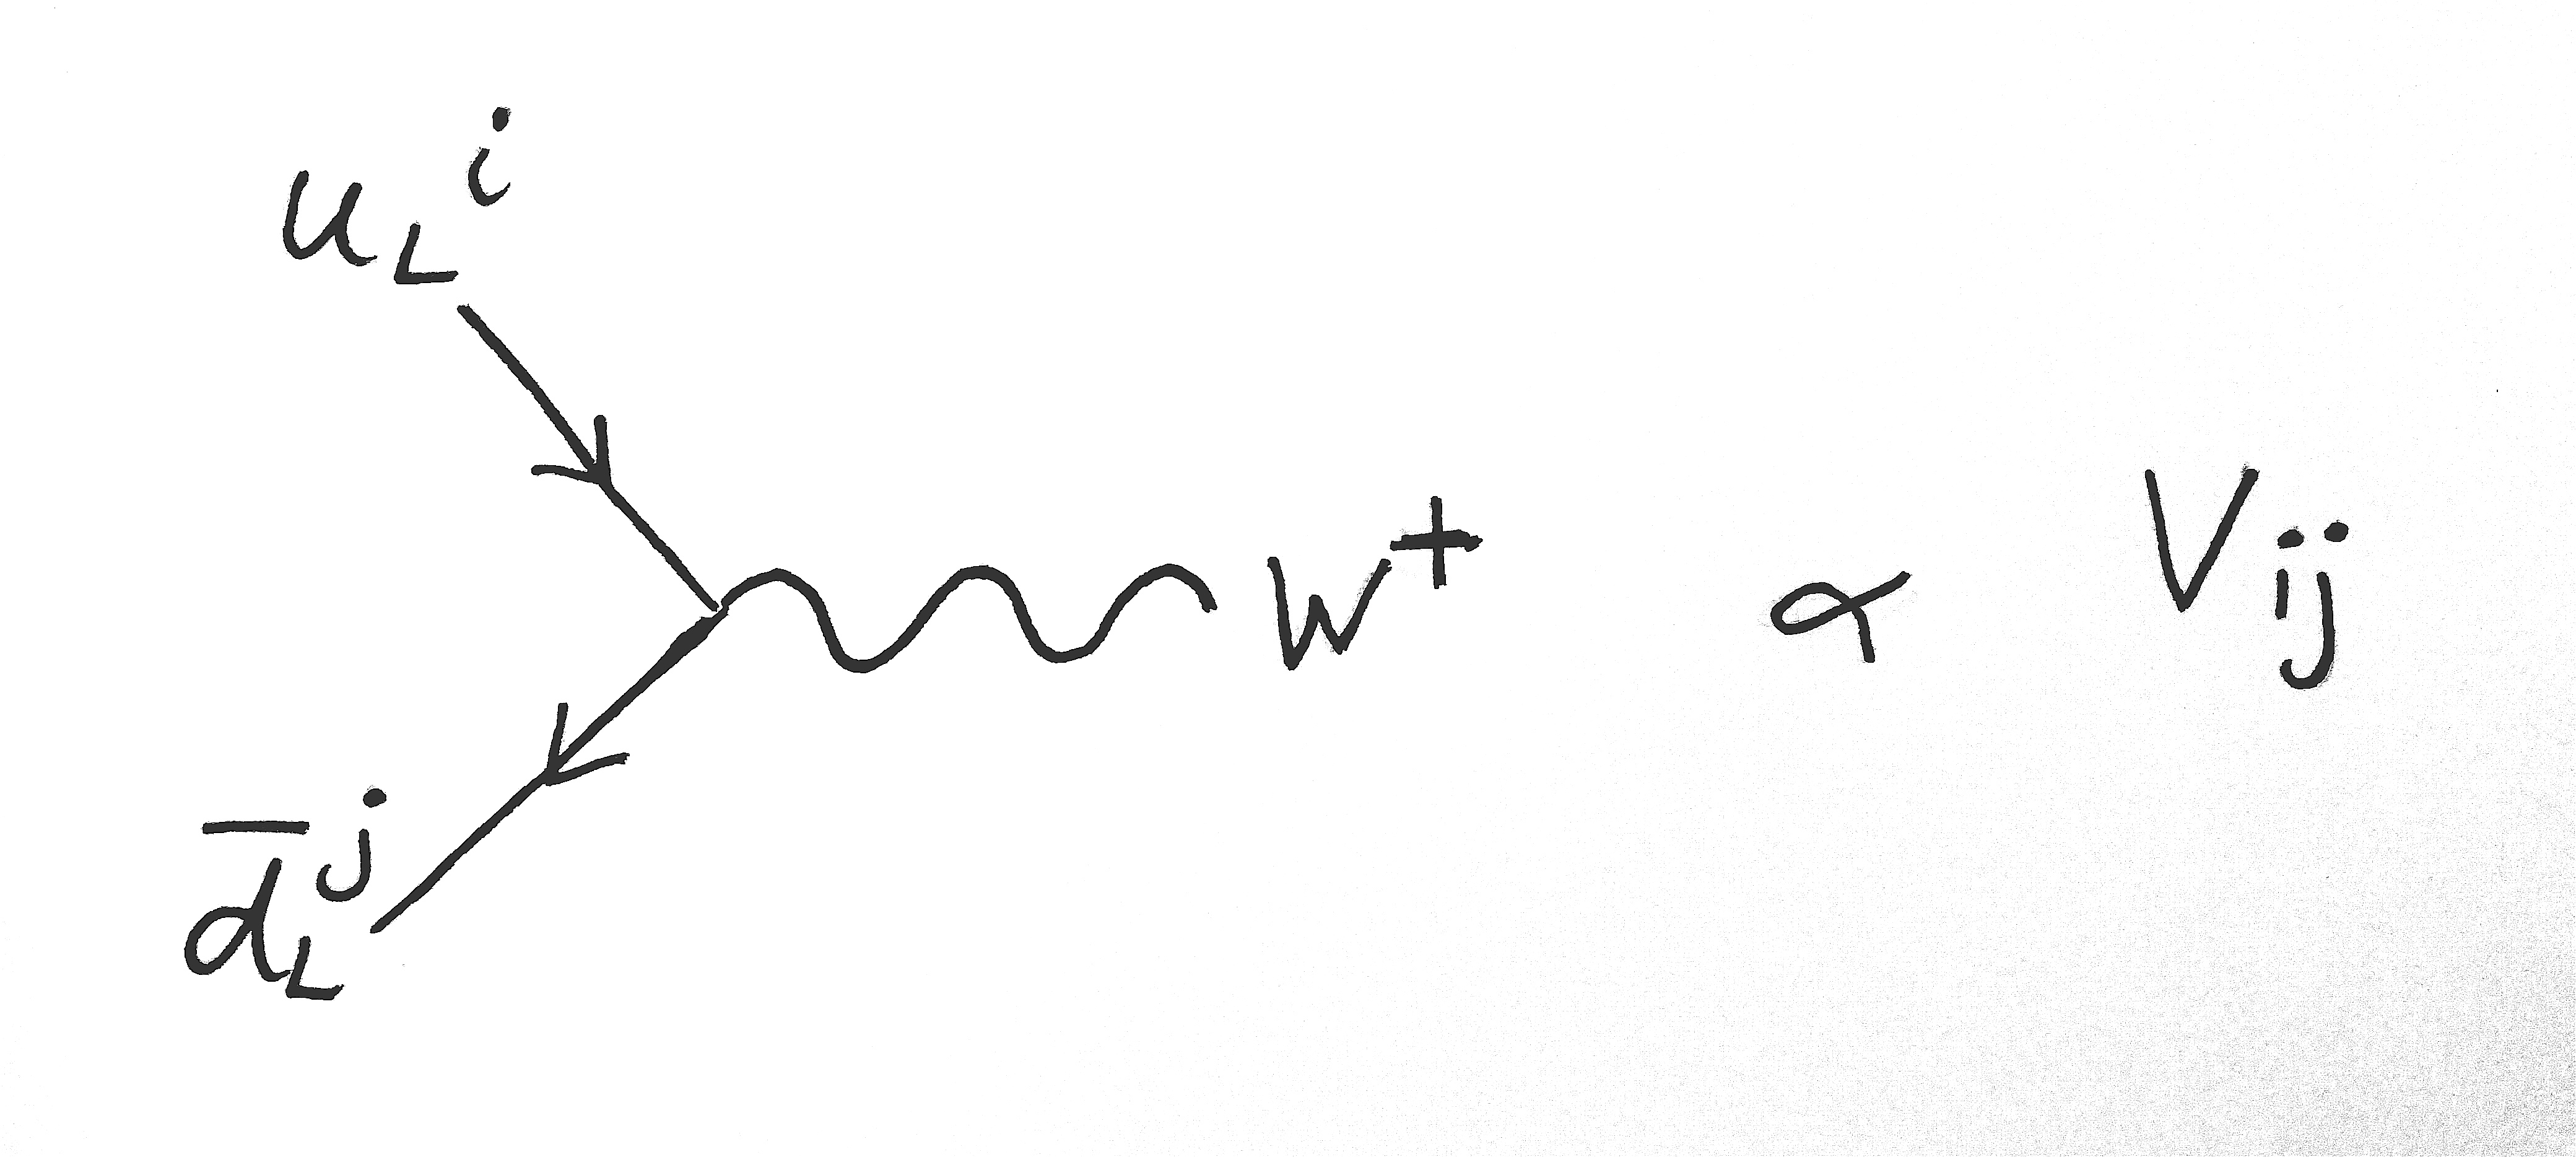
\includegraphics[width=0.5\textwidth]{images/fccc.jpg}
    \vspace{-10pt}
  \end{center}
  \caption{The flavor-changing charged current vertex.}
  \label{fig:fccc}
\end{figure}

We can now turn to the physical consequences of $\mathcal{L}_{\text{FCCC}}$. The interactions given in this part of the Lagrangian describe a quark changing flavor while emitting a $W^{\pm}$ boson (Fig. \ref{fig:fccc}). The propensity for flavor $i$ to decay into another flavor $j$ is governed in part by energy constraints and in part by the associated CKM element $V_{ij}$. These quark-level interactions mediate meson decays, namely leptonic and semileptonic decays, described in Sec. \ref{sec:weakdecays}.

The deviation of $V_{ij}$ from a unit matrix breaks some of the symmetries of the SM. $\mathcal{L}_{\text{SM}}-\mathcal{L}_{\text{FCCC}}$ has the property that one can independently rephase each of the quark fields, $q_i\to e^{i\theta_i}q_i$, a global $U(1)$ symmetry for each quark flavor. This implies, via Noether's theorem, that the number of quarks of each flavor, $N_i$, is conserved. However, $\mathcal{L}_{\text{FCCC}}$ breaks this symmetry $U(1)^6\to U(1)$. There is only a remnant symmetry of transforming all flavors by the same phase. Individual quark flavor number is no longer conserved, but overall quark number is.

Since there is no off-diagonal flavor structure for the leptons, the equivalent global $U(1)^6$ symmetry for the leptons survives in the SM. Individual lepton flavor number is conserved. This property of the SM is referred to as lepton flavor universality.

\subsection{CKM Matrix Unitarity}

The exact values of the CKM matrix elements are of interest in the search for new physics. The CKM matrix is unitary by construction. However, we may discover that the values we measure experimentally do not combine to produce a unitary matrix. This would be evidence that the elements we are measuring, in fact, compose a submatrix of a unitary matrix larger than $3\times 3$. This would imply the presence of further, heavier quark generations. Below once again I follow \cite{Schwartz:2013pla}.

%% Another source of interest in the CKM values is CP violation. CP violation is a global symmetry exhibited by $\mathcal{L}_{\text{SM}}-\mathcal{L}_{\text{FCCC}}$, and physically corresponds to a symmetry between particles and antiparticles. CP violation is one of the famous {\it{Sakarov conditions}}, the conditions necessary for a theory to explain the matter/antimatter asymmetry observed in the universe. CP is generically violated when a parameter of the theory has an imaginary component. The CKM matrix contains one physical phase, making $\mathcal{L}_{\text{FCCC}}$ a source of CP violation. However, the extent of CP violation in the flavor sector is not sufficient to explain the matter/antimatter asymmetry, so the necessary CP violating processes will likely come from new physics beyond the standard model.


%% To understand the structure of the CKM, we must first ask how many independent physical parameters there are. If one imagines that $V$ is purely real, then it becomes an $SO(3)$ matrix, which can be parameterized by 3 angles, so there are $N_{\text{real}} = 3$ independent real parameters. A member of $SU(3)$ has 9 independent parameters, so there must be $N_{\text{im}}=N-N_{\text{real}} = 6$ independent phases.

%% However, we have the freedom to remove some of those phases via a redefinition of the quark fields. $\mathcal{L}_{\text{SM}} - \mathcal{L}_{\text{FCCC}}$ has a global $U(1)^6$ symmetry, a rephasing of each of the 6 quark flavors. One can rephase each flavor without modifying $\mathcal{L}_{\text{SM}} - \mathcal{L}_{\text{FCCC}}$, but with the effect of changing $V$:
%% \begin{align}
%%   V \,\,\to \,\,
%%   \begin{pmatrix}
%%     e^{-ia} & 0 & 0 \\
%%     0 & e^{-ib} & 0 \\
%%     0 & 0 & e^{-ic} \\
%%   \end{pmatrix}
%%   V
%%   \begin{pmatrix}
%%     e^{id} & 0 & 0 \\
%%     0 & e^{ie} & 0 \\
%%     0 & 0 & e^{if} \\
%%   \end{pmatrix},
%% \end{align}
%% where $a,b,c,d,e,f\in \mathbb{R}$. So perhaps one can tune each of these 6 phases to remove all 6 phases in $V$. This is not quite right, we in fact only have the ability to remove 5 of the 6 phases. To see why we can redefine the phases in the following way;
%% \begin{align}
%%   V \,\,\to \,\,
%%   \begin{pmatrix}
%%     e^{-ia} & 0 & 0 \\
%%     0 & e^{-i(a+\alpha)} & 0 \\
%%     0 & 0 & e^{-i(a+\beta)} \\
%%   \end{pmatrix}
%%   V
%%   \begin{pmatrix}
%%     e^{i(a+\gamma)} & 0 & 0 \\
%%     0 & e^{i(a+\delta)} & 0 \\
%%     0 & 0 & e^{i(a+\epsilon)} \\
%%   \end{pmatrix},
%% \end{align}
%% with $\alpha,\beta,\gamma,\delta,\epsilon\in\mathbb{R}$. $a$ is a useless phase - it will always cancel with itself so cannot be used to remove a phase from $V$. Hence, one can remove 5 of the 6 phases by redefining the quark fields, leaving one physical phase in the CKM matrix.

%% This is can be seen as due to the explicit symmetry breaking property of $\mathcal{L}_{\text{FCCC}}$. The inclusion of $\mathcal{L}_{\text{FCCC}}$ breaks the global $U(1)^6$  symmetry down, $U(1)^6 \to U(1)$, where the broken symmetry is a rephasing of all of the quark flavors by the same amount. This says we can modify $\mathcal{L}_{\text{FCCC}}$ by $N_{\text{broken}} = 5$ independent phases without modifying the rest of the Lagrangian.

%% The CKM contains 3 real parameters and 1 complex phase. There is only one complex phase since we can freely redefine the phases of the quark fields in order to absorb the majority of the phases in the CKM. A common parameterisation is
%% \begin{align}
%%   V =
%%   \begin{pmatrix}
%%     1 & 0 & 0 \\
%%     0 & \cos\theta_{23} & \sin\theta_{23} \\
%%     0 & -\sin\theta_{23} & \cos\theta_{23} \\
%%   \end{pmatrix}
%%   \begin{pmatrix}
%%     1 & 0 & \sin\theta_{12}e^{i\delta} \\
%%     0 & 1 & 0  \\
%%     -\sin\theta_{13} e^{i\delta} & 0 & \cos\theta_{13} \\
%%   \end{pmatrix}
%%   \begin{pmatrix}
%%     \cos\theta_{12} & \sin\theta_{12} & 0  \\
%%     -\sin\theta_{12} & \cos\theta_{12} & 0 \\
%%     0 & 0 & 1 \\
%%   \end{pmatrix}.
%% \end{align}
%% A useful parameterisation for understanding the relative sizes of the CKM elements is due to Wolfenstein. Define the Wolfenstein parameter $\lambda = \sin\theta_{12}$, which is known experimentally to be around $\lambda\simeq 0.22$. Then $\cos\theta_{12} = \sqrt{1-\sin^2\theta_{12}} = \sqrt{1-\theta^2} \simeq 1 - \lambda^2/2$. Observing then that $\sin\theta_{23} \sim 0.04 \simeq \lambda^2$ and $\sin\theta_{13} \sim 0.004 \simeq \lambda^3/3$, we can write the matrix as
%% \begin{align}
%%   V \simeq
%%   \begin{pmatrix}
%%     1 - {1\over 2}\lambda^2 & \lambda & {1\over 3} \lambda^3 e^{i\delta}  \\
%%     - \lambda & 1 - {1\over 2}\lambda^2 & \lambda^2 \\
%%     \lambda^3(1-{1\over3} e^{i\delta}) & -\lambda^2 & 1 \\
%%   \end{pmatrix}
%%   =
%%   \begin{pmatrix}
%%     \order{1} & \order{\lambda} & \order{\lambda^3}  \\
%%     \order{\lambda} & \order{1} & \order{\lambda^2} \\
%%     \order{\lambda^3} & \order{\lambda^2} & \order{1} \\
%%   \end{pmatrix}
%% \end{align}
%% There is a clear hierarchy between the values - the CKM matrix is close to the unit matrix. Inter-generational mixing is dominant, dropping from second to first generation is suppressed by $\lambda$, dropping from third to second by $\lambda^2$, and dropping from third to first by $\lambda^3$. The SM supplies no compelling explaination of why this hierarchy exists, it is expected that new physics beyond the SM will supply some natural explaination.

\begin{figure}
  \vspace{-10pt}
  \begin{center}
    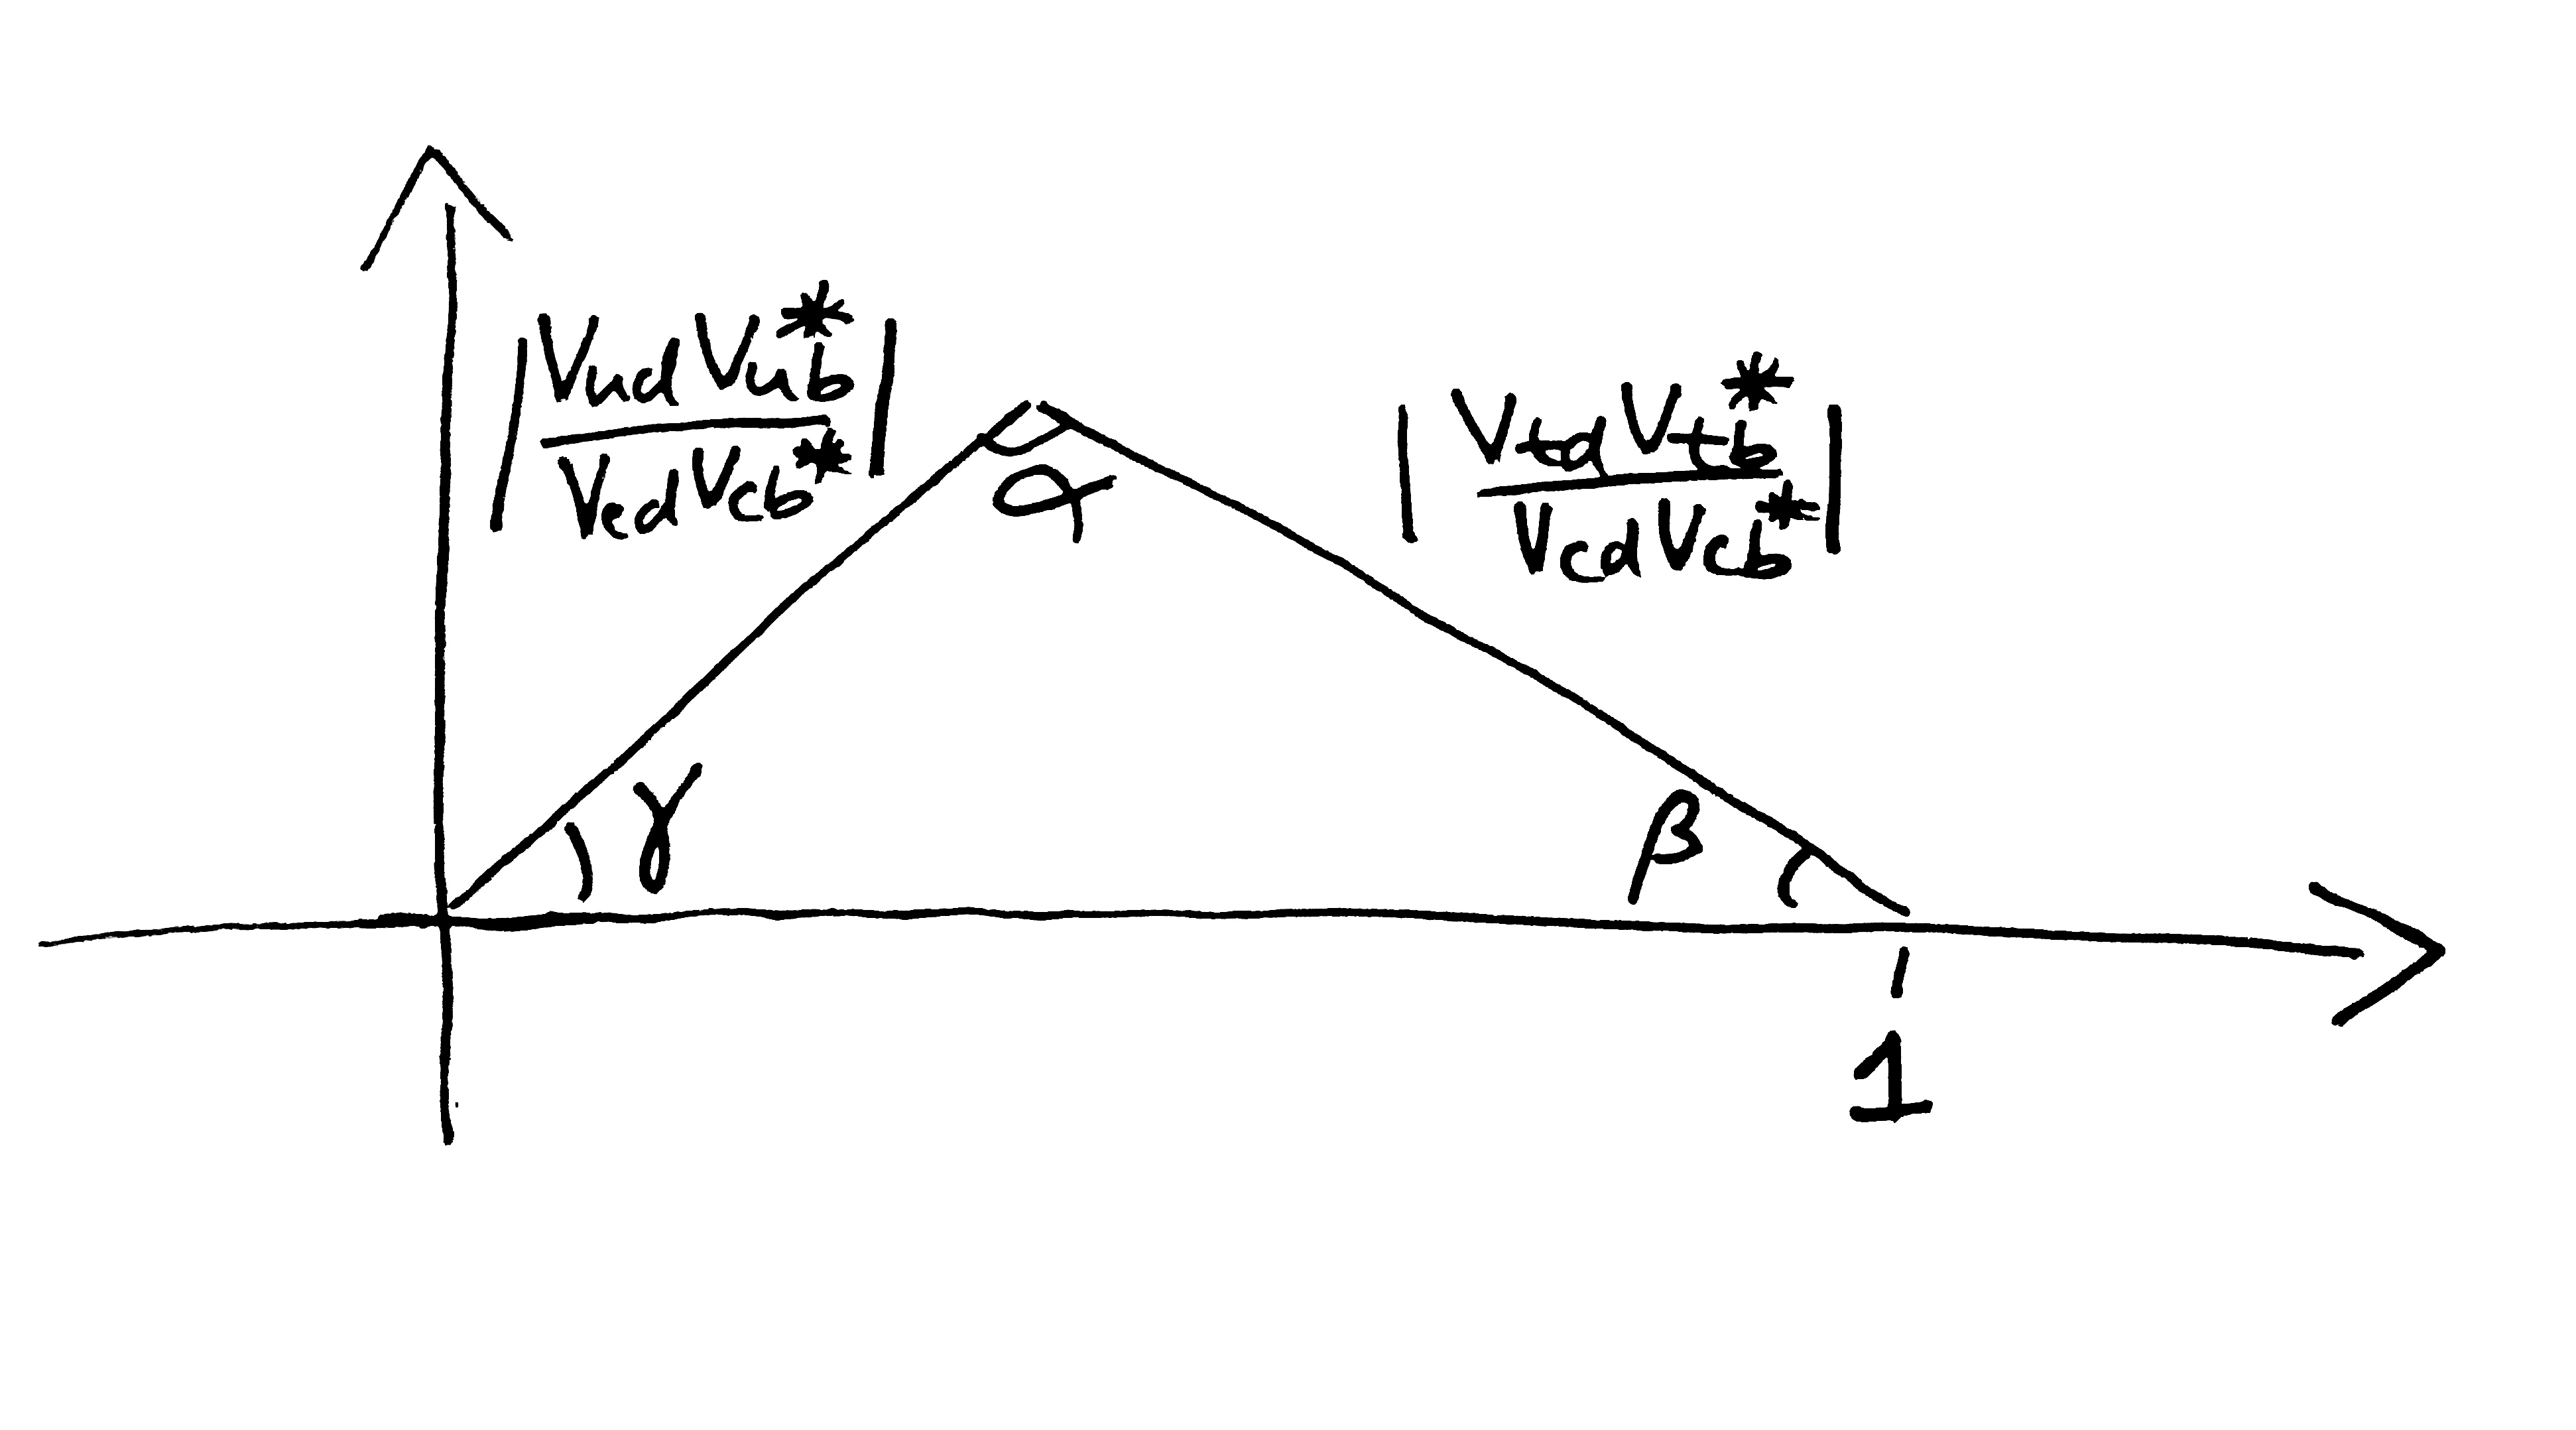
\includegraphics[width=0.7\textwidth]{images/unitaritytriangle_sketch.jpg}
  \end{center}
  \vspace{-40pt}
  \caption{A sketch of the unitarity triangle.}
  \label{fig:unitaritytriangle_sketch}
\end{figure}

The assumption of unitarity in $V$:
\begin{align}
  V_{ji}^*V_{jk}=\delta_{ik},
  \label{eq:CKMunitarity}
\end{align}
imposes 9 constraints on the CKM elements. Each of these constraints gives a test of the SM. If one of these constraints is found to be violated, this would represent evidence of new physics. The most studied constraint is given by taking $i=3,k=1$:
\begin{align}
  {V_{ud}V_{ub}^*\over V_{cd} V_{cb}^*} + {V_{td}V_{tb}^* \over V_{cd}V_{cb}^*} + 1 = 0.
\end{align}
This can be visualized as a triangle (known as the {\it{unitarity triangle}}) on the complex plane, as shown in Fig. \ref{fig:unitaritytriangle_sketch}.

For unitarity, the triangle must close, in other words, $\alpha+\beta+\gamma = \pi$. Hence one test of CKM unitarity is to measure these angles
\begin{align}
  \alpha = \arg \left( -{V_{td}V_{tb}^*\over V_{ud}V_{ub}^*}\right) \,,\,
  \beta = \arg \left( -{V_{cd}V_{cb}^*\over V_{td}V_{tb}^*} \right) \,,\,
  \gamma = \arg \left( -{V_{ud}V_{ub}^*\over V_{cd}V_{cb}^*} \right).
\end{align}
These angles can be constructed from measured CKM elements. They can also be measured directly from certain processes, for example $\gamma$ can be measured by studying $B\to DK$ decays \cite{GRONAU1991172,GRONAU1991483}. The unitarity triangle also contains information about CP-violation from flavor-changing charged currents. The Jarlskog invariant%, $J=\sin\theta_{12}\sin\theta_{23}\sin\theta_{31}\cos\theta_{12}\cos\theta_{23}\cos\theta_{31}^2\sin\delta$,
, a measure of CP-violation, is proportional to the area enclosed by the triangle.

The most recent PDG update \cite{PhysRevD.98.030001} reports the following averages for the measurements of CKM elements:
\begin{align}
  |V| = \begin{pmatrix}
    0.97446\pm 0.00010 & 0.22452\pm 0.00044 & 0.00365\pm 0.00012 \\
    0.22438\pm 0.00044 & 0.97359\substack{+0.00010\\-0.00011} & 0.04214\pm 0.00076 \\
    0.00896\substack{+0.00024\\-0.00023} & 0.04133\pm 0.00074 & 0.999105\pm 0.000032 \\
  \end{pmatrix}.
\end{align}
The averages given here are consistent with unitarity in all avaliable tests. The element we are most interested in in this thesis is $|V_{cb}| = 0.04214\pm 0.00076$, this is the second least precise of the determinations at present. %For example, taking \eqref{eq:CKMunitarity} with $i=k=1$, we find $|V_{ud}|^2+|V_{us}|^2+|V_{ub}|^2 = 0.9994\pm 0.0005$.
The angles of the unitarity triangle currently satisfy $\alpha+\beta+\gamma = (180\pm 7)\degree$. Increasing the precision of CKM determinations is necessary to provide more stringent tests of CKM unitarity.

\begin{figure}
  \vspace{-10pt}
  \begin{center}
    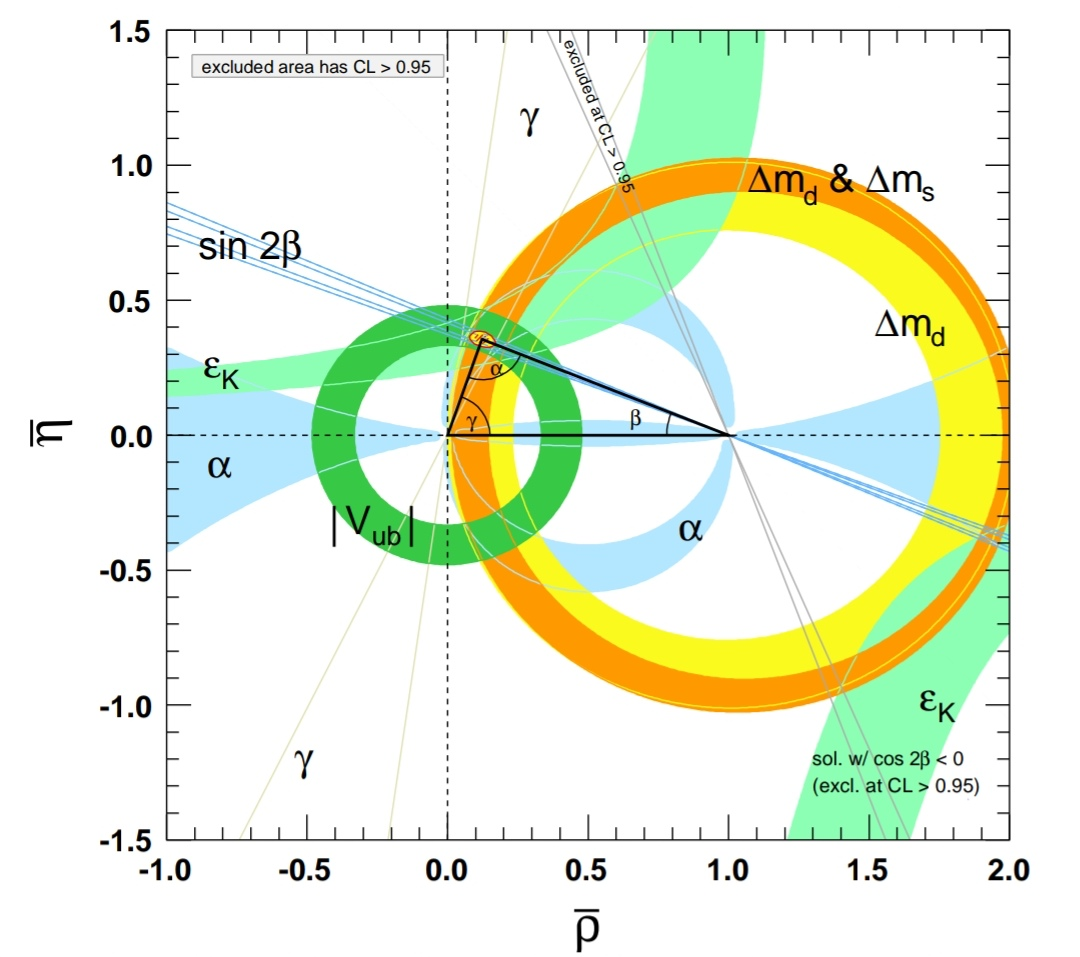
\includegraphics[width=0.6\textwidth]{images/ckmpdg.jpg}
  \end{center}
  \vspace{-15pt}
  \caption{Exclusion regions for the vertices of the CKM triangle from various measurements, coutresy of the most recent PDG update \cite{PhysRevD.98.030001}.}
  \label{fig:ckmpdg}
\end{figure}

\subsection{Weak Decays}
\label{sec:weakdecays}

I now move on to the methods of determining CKM elements, following discussion in \cite{Fleischer:2006fx}. At the confinement scale ($\sim$1GeV and below), quarks are confined by QCD in hardons. At these energies, the dynamics of quarks are only experimentally accessible by probing the dynamics of hadrons. CKM matrix elements are determined by studying hadron decays.

First some definitions of hadron classification. Hadrons are categorized into mesons (charged with one valence quark and one valence antiquark) and baryons (three valence quarks). The entirety of this thesis is concerned with mesons. Mesons are categorized in terms of the flavors they are charged under and their representations under the Lorentz group. We use the same notation as for the quantum numbers of the weak currents; $L^{\pm}$ where $L$ denotes spin and $\pm$ denotes parity. In this thesis, we are concerned mostly with pseudoscalar ($0^-$) and vector ($1^-$) mesons.

Weak decays of mesons are categorized according to the final products:
\begin{itemize}
\item
  {\bf{Leptonic}}: $meson \to leptons$.
\item
  {\bf{Semileptonic}}: $meson \to meson + leptons$.
\item
  {\bf{Hadronic}}: $meson \to mesons$.
\item
  {\bf{Oscillation}}: $meson \to meson$.
\end{itemize}

All of these types of decay are dependent on CKM elements so can in principle to be used for studying them. We are most interested in the first two, leptonic and semileptonic, so will give detail of such decays here.

\begin{figure}
  \vspace{-10pt}
  \begin{center}
    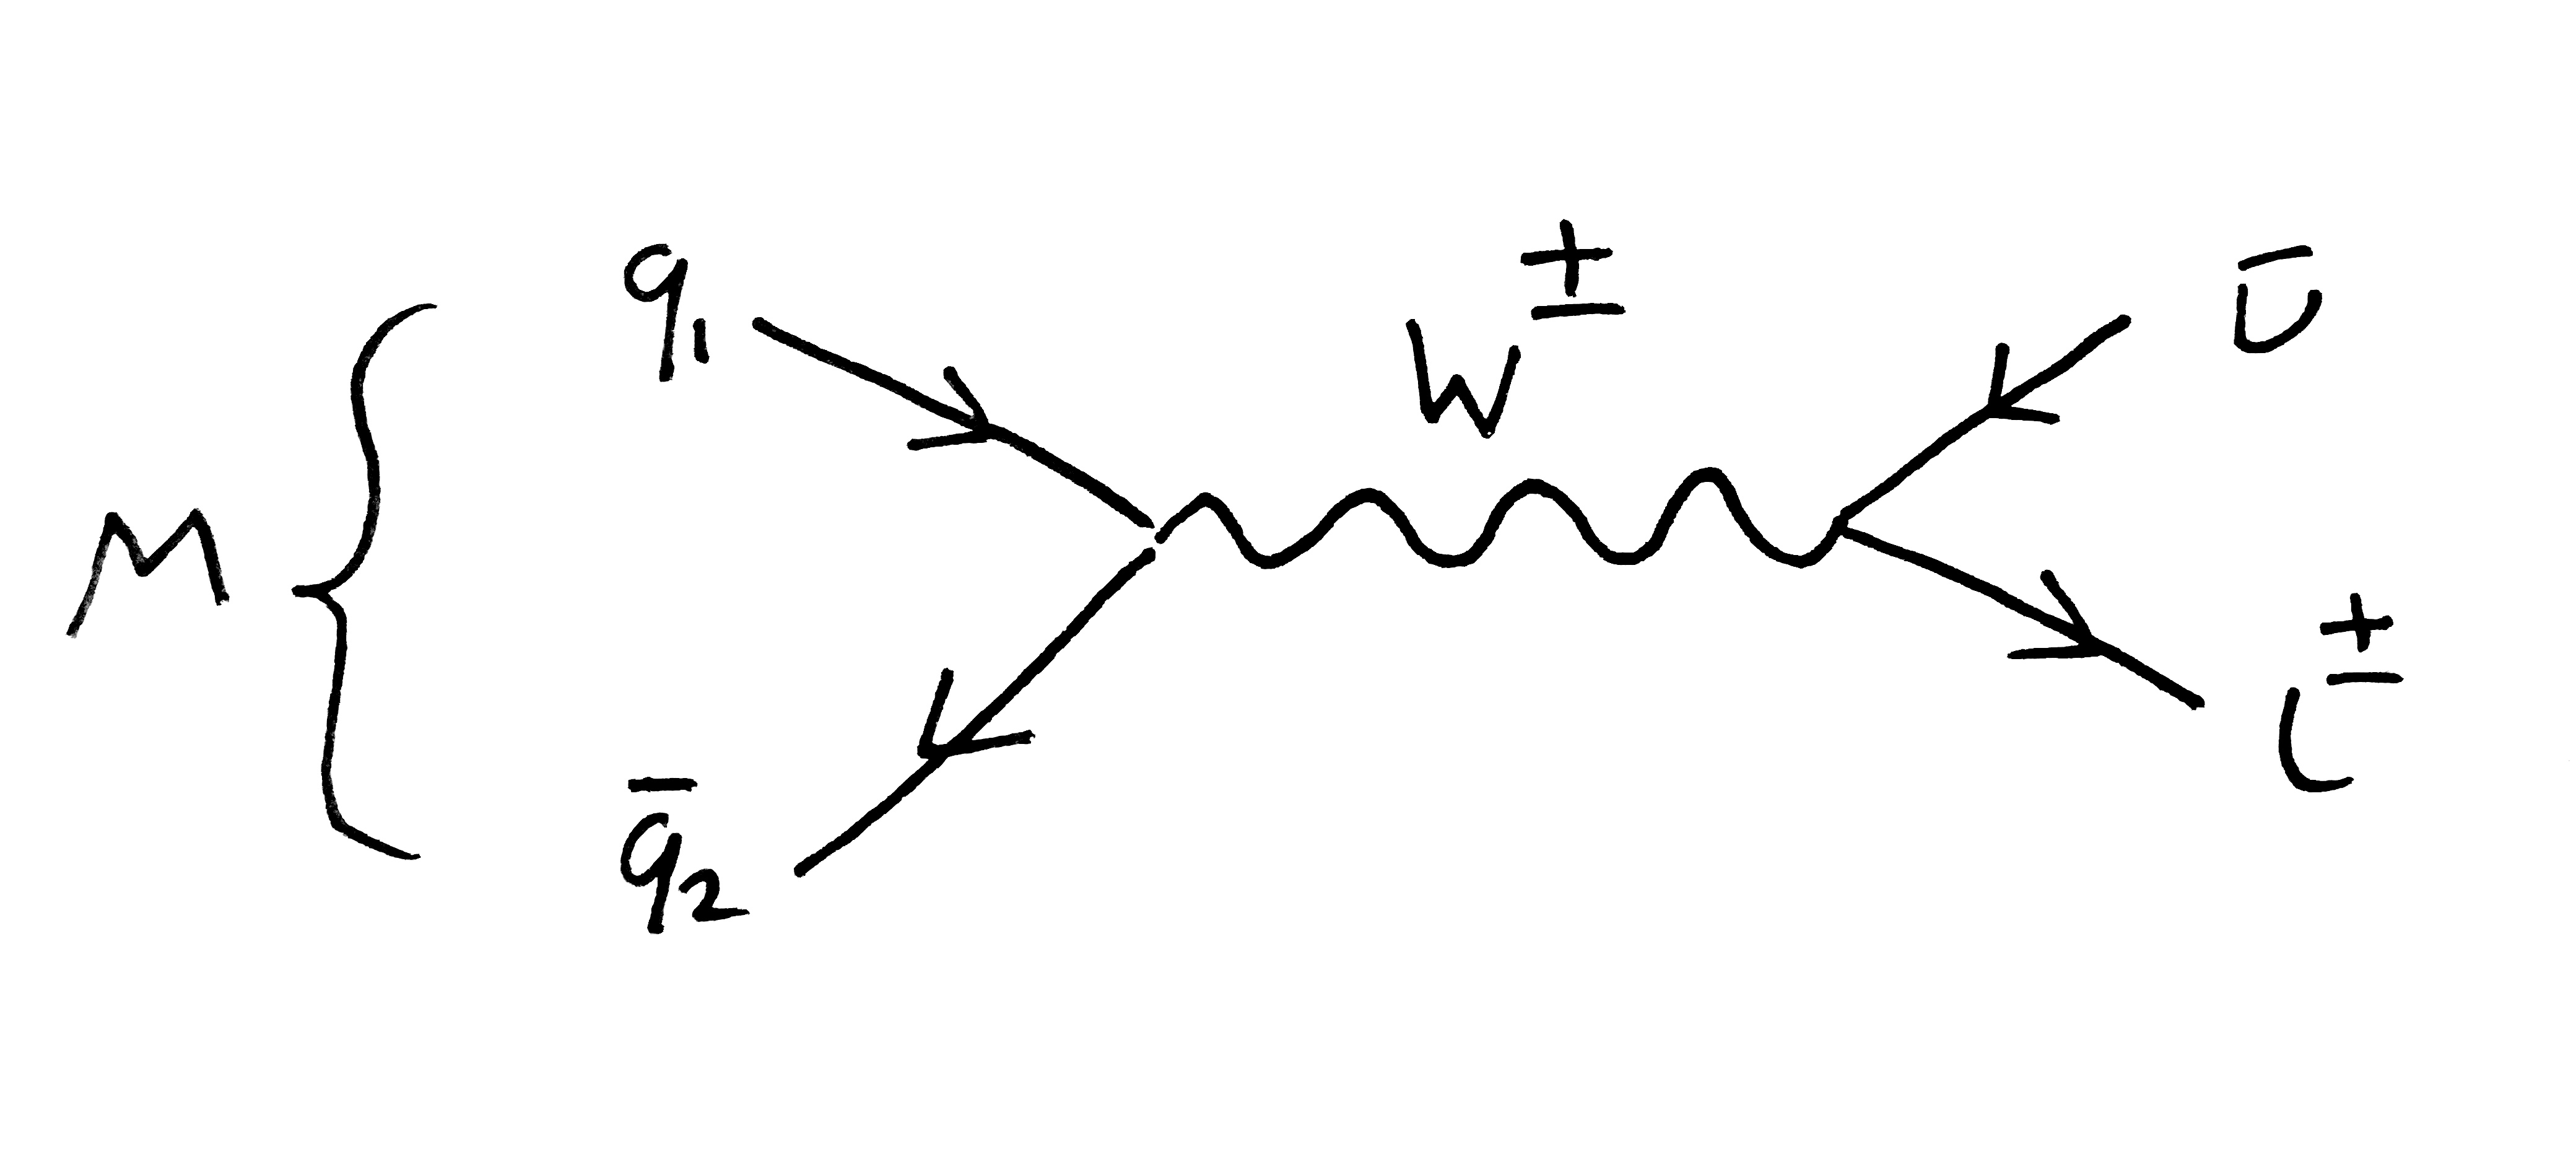
\includegraphics[width=0.6\textwidth]{images/leptonicdecay.jpg}
  \end{center}
  \vspace{-20pt}
  \caption{Leptonic decay of meson $M$ at tree level in the electroweak coupling.}
  \label{fig:leptonicdecay}
\end{figure}

Fig. \ref{fig:leptonicdecay} shows a generic leptonic decay at tree level in electroweak coupling (virtual quark and gluon lines are implicit). The corresponding amplitude is given by
\begin{align}
  \mathcal{M} = \left({ie\over \sqrt{2}\sin\theta_W}\right) V_{q_1q_2} \langle l\bar{\nu} | L^l_{\mu} D_W^{\mu\nu} J_{\nu}^{q_1q_2} | M \rangle,
\end{align}
where $D_{W}$ is a free $W^{\pm}$ propagator, $|M\rangle$ is the ground state of the meson $M$, and $|l\bar{\nu}\rangle$ is a lepton-antineutrino state. We are using the notation $L^l_{\mu}=L^{kk}_{\mu}$, where $l$ indexes the $k$th charged lepton. If the momentum of the meson, $p^2$, is much smaller than the $W$ mass squared, one can integrate out the dynamics of the $W$ resulting in Fermi effective theory:
\begin{align}
  \nonumber
  \left({ie\over\sqrt{2}\sin\theta_W}\right)^2 D^{\mu\nu}_W(p^2) &= \left({ie\over\sqrt{2}\sin\theta_W}\right)^2 \left( -ig^{\mu\nu} \over p^2 - M_W^2 \right)
  \\ & = \underbrace{ {i\over M_W^2} \left( ie \over \sqrt{2}\sin\theta_W \right)^2  }_{\equiv -2\sqrt{2}G_F} g^{\mu\nu} + \mathcal{O}\left({p^2\over M_W^4}\right).
\end{align}
Then $\mathcal{M}$ can be factorised;
\begin{align}
  \mathcal{M} \simeq -2\sqrt{2} G_F V_{q_1q_2} \langle l\bar{\nu} | L_{\mu}^l | \Omega \rangle \langle \Omega | J^{q_1q_2\, \mu} | M \rangle.
\end{align}
$\langle \Omega | J^{q_1q_2}_{\mu}| M \rangle$ is a non-perturbative quantity, since it concerns the transitions of a strongly coupled bound state (QCD at the confinement scale). We know that it has a Lorentz index $\mu$, and the only Lorentz vector in the system is the meson's 4-momentum $p_{\mu}$. So we define
\begin{align}
  \langle\Omega | J_{q_1q_2}^{\mu} | M \rangle = p^{\mu} f_M,
  \label{eq:decay_constant_def}
\end{align}
where $f_M$ is a Lorentz invariant known as the {\it{decay constant}} of the meson $M$, and encodes all non-perturbative information in the amplitude.

By taking the modulus squared of $\mathcal{M}$ and integrating over all allowed momenta of the final state, one finds the decay rate of the process;
\begin{align}
  \Gamma(M\to l\bar{\nu}) = {G_F^2\over 8\pi} f_M^2 m_{\ell}^2 M_M \left( 1 - {m_{\ell}\over M_M^2} \right)^2 |V_{q_1q_2}|^2\,.
\end{align}
$m_{\ell}$ here is the mass of the final state charged lepton. In order to find $|V_{q_1q_2}|$, one requires both a measurement of $\Gamma(M\to l\bar{\nu})$, and a value for $f_M$. $f_M$ can be computed in a lattice QCD calculation.

%\begin{wrapfigure}{R}{0.55\textwidth}
\begin{figure}
  \vspace{-10pt}
  \begin{center}
    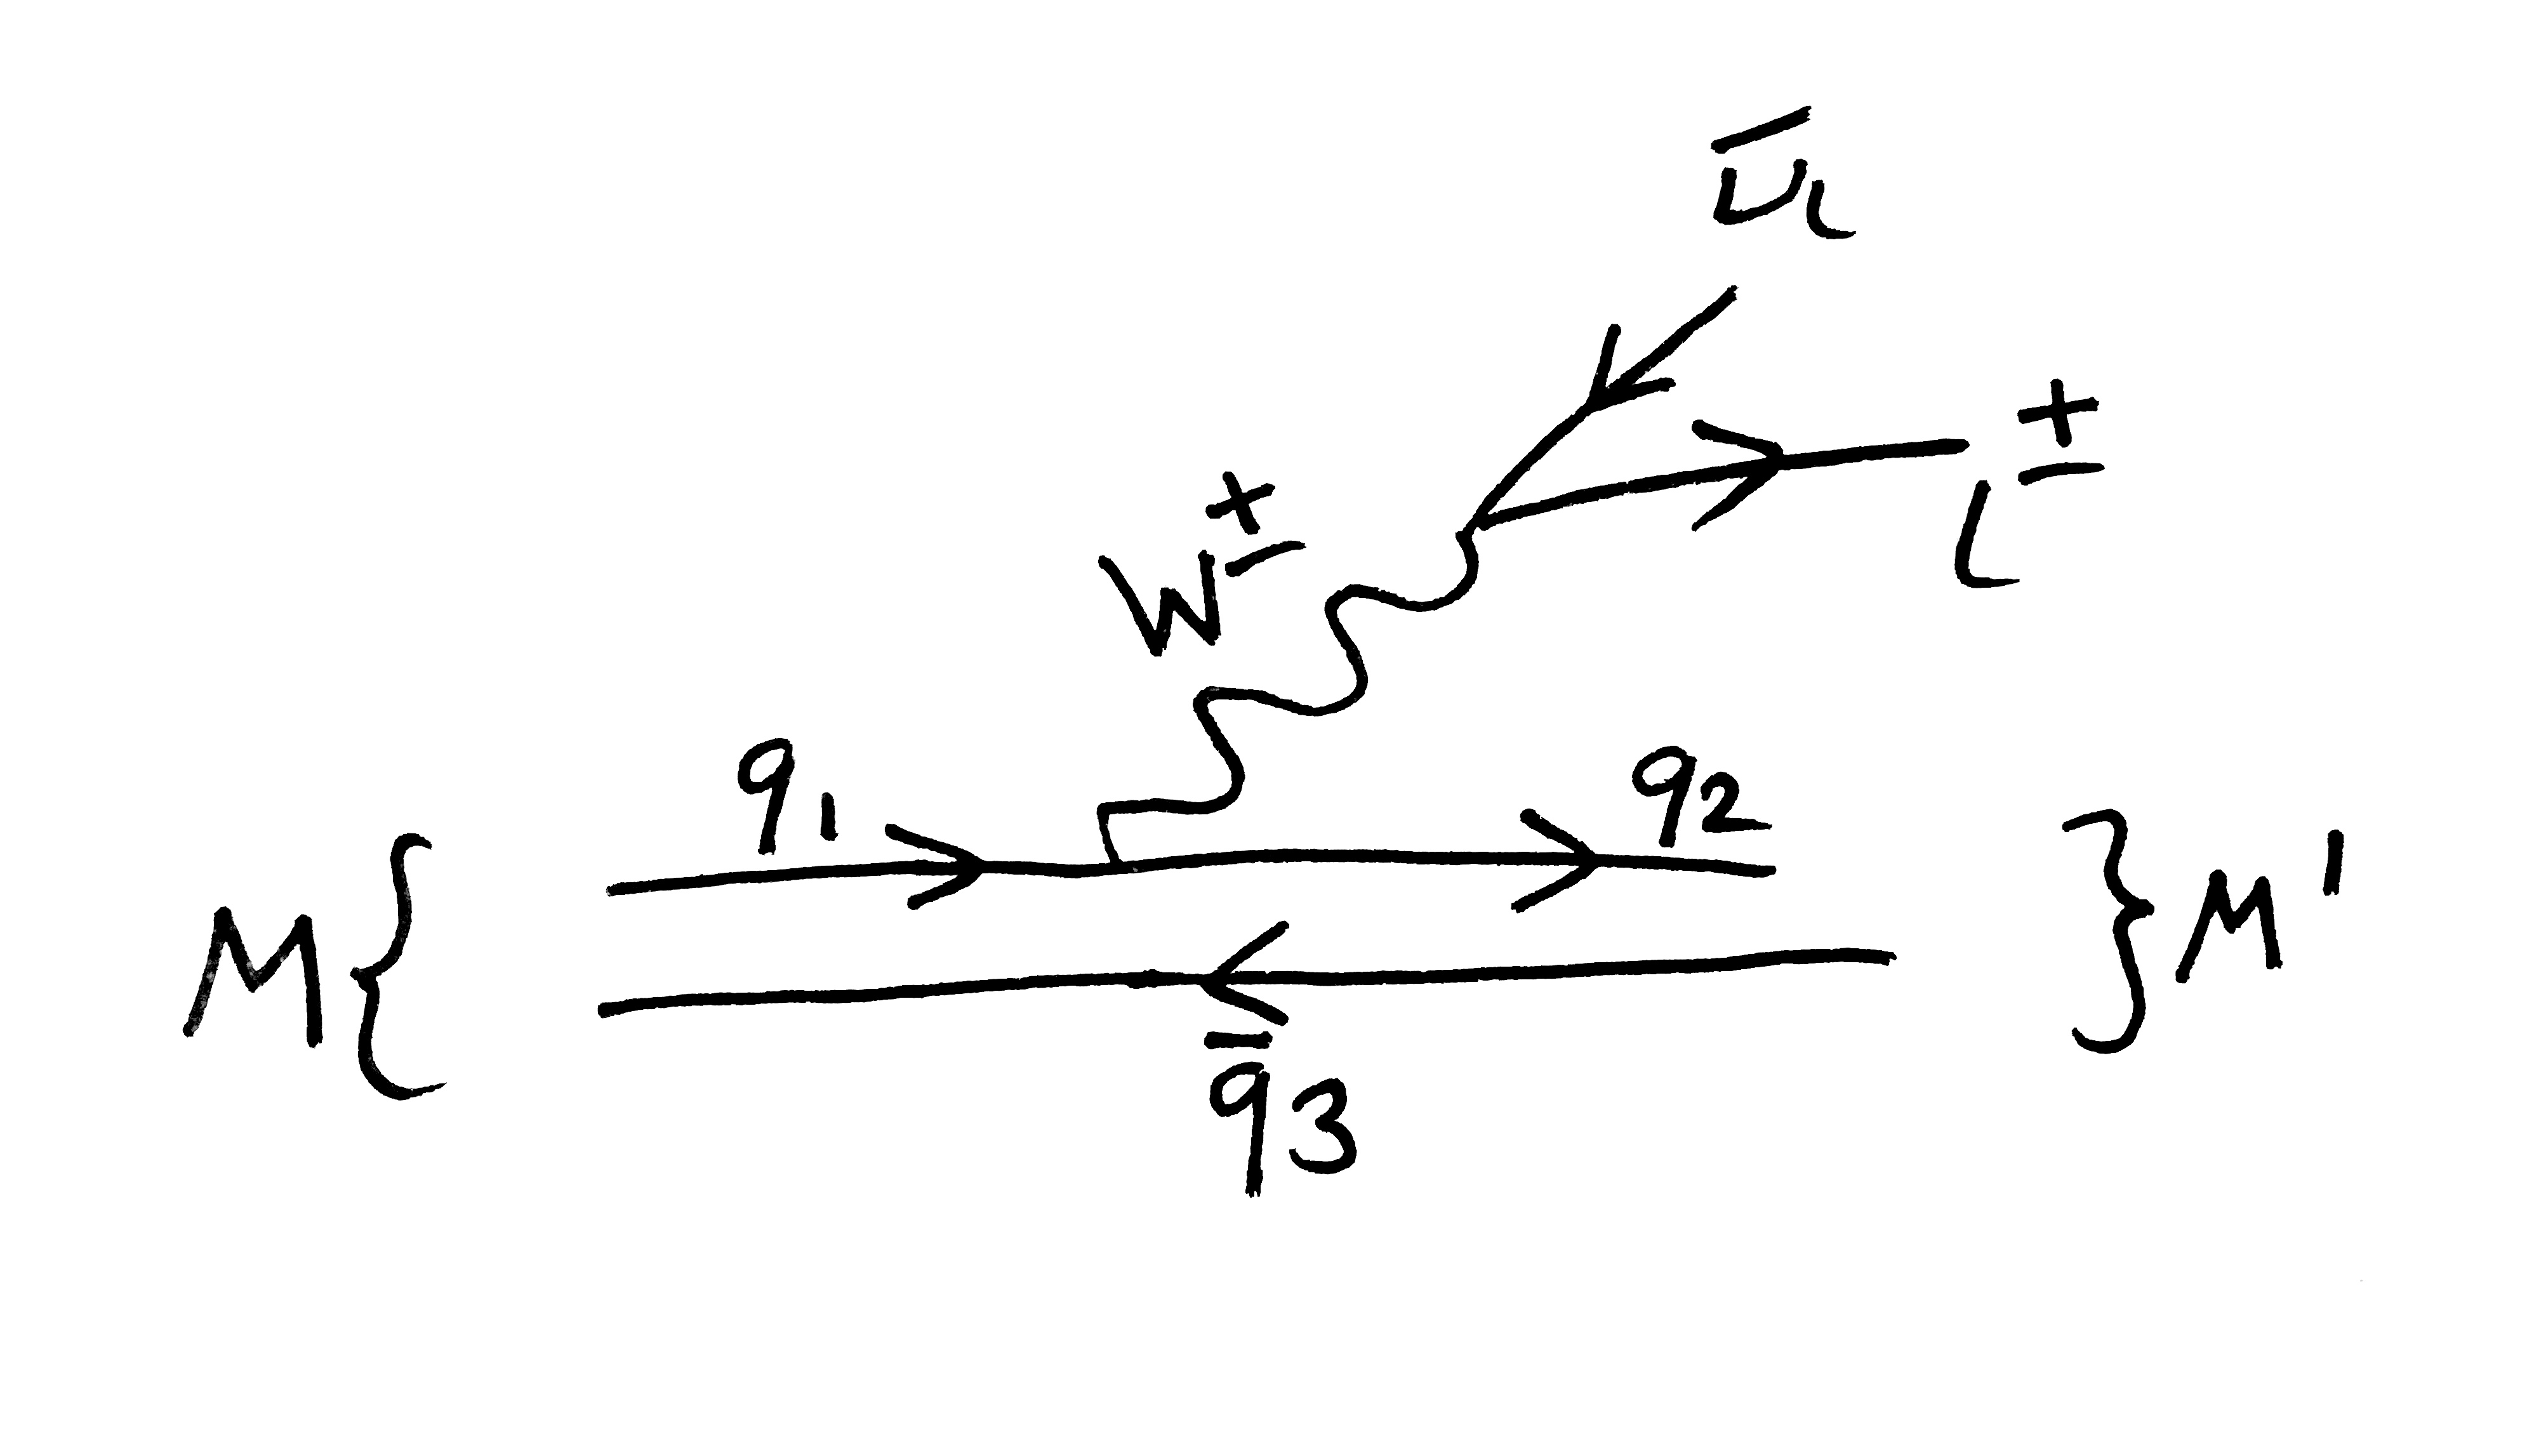
\includegraphics[width=0.6\textwidth]{images/semileptonicdecay.jpg}
  \end{center}
  \vspace{-30pt}
  \caption{Semileptonic decay, $M\to M'l\bar{\nu}$, at tree level in electroweak coupling.}
  \label{fig:semileptonicdecay}
\end{figure}
%\end{wrapfigure}

A similar story accompanies semileptonic decays. A typical semileptonic decay (at tree level in the electroweak coupling) is depicted in Fig. \ref{fig:semileptonicdecay}. The amplitude is given by
\begin{align}
  \nonumber
  \mathcal{M} & = \left( { ie \over \sqrt{2} \sin\theta_W }\right) V_{q_1q_2} \langle M', l\bar{\nu} | J_{\mu}^{q_1q_2} D_W^{\mu\nu} L^l_{\nu} | M \rangle\,, \\
  \nonumber
  & \simeq -2\sqrt{2} G_F V_{q_1q_2} \langle M', l\bar{\nu} | J_{\mu}^{q_1q_2} L^{l\, \mu} | M \rangle\,, \\
  & \simeq -2\sqrt{2} G_F V_{q_1q_2} \langle l\bar{\nu} | L^{l\,\mu} | \Omega \rangle \langle M' | J_{\mu}^{q_1q_2} | M \rangle,
  \label{eq:semileptonic}
\end{align}
where on the second line we have integrated out the $W$ propagator by using the same expansion as in the leptonic case, and on the third line we have factorised the QCD part from the electroweak part. The matrix element $\langle M' | J_{\mu}^{q_1q_2} | M \rangle$ is a non-perturbative quantity. Unlike in the previous case, there are a number of ways one can choose to parameterise this matrix element, and appropriate choices vary depending on the quantum numbers of $M$ and $M'$. Of interest to us are the cases where $M$ is a pseudoscalar meson $0^-$, and $M'$ is either pseudoscalar or vector $1^-$.

In the {\bf{pseudoscalar$\to$pseudoscalar}} case, only the vector component of the current survives in the matrix element, $\langle M' | J_{\mu}^{q_1q_2} | M \rangle = \langle M' | V_{\mu}^{q_1q_2} | M \rangle$. $\,\,\langle M' | A_{\mu}^{q_1q_2} | M \rangle$ vanishes since this does not respect the parity invariance of QCD (it has negative parity). The most popular parameterisation of $\langle M' | V_{\mu}^{q_1q_2} | M \rangle$ is
\begin{align}
  \langle M' | V_{\mu}^{q_1q_2} | M \rangle = f_+(q^2) \left[ P_{\mu} + p_{\mu} - {M^2-m^2\over q^2} q_{\mu} \right]  + f_0(q^2) {M^2-m^2\over q^2} q_{\mu}.
  \label{eq:formfactors_experimental}
\end{align}
$M,P_{\mu}$ are the $M$-meson mass and momentum and $m,p_{\mu}$ are the $M'$-meson mass and momentum. $f_0(q^2)$ and $f_+(q^2)$, known as the scalar and vector form factors, encoding all non-perturbative information. We now have non-perturbative functions of $q^2$ rather than a single number. $q^2=(P-p)^2$, the momentum carried away from the meson by the $W$, has an allowed range of values if the final states are on-shell (obey the classical dispersion relation):
\begin{align}
  m_{\ell}^2 \leq q^2 \leq (M-m)^2.
\end{align}
By integrating $|\mathcal{M}|^2$ over all final lepton and neutrino momenta, one finds a differential decay rate,
\begin{align}
  {d\Gamma\over dq^2}(M\to M'l\bar{\nu}) =& \eta_{\text{EW}} { G_F^2 |V_{q_1q_2}|^2\over 24 \pi^3 M^2 } \left( 1 - {m_{\ell}^2\over q^2}\right)^2 |{\bf{p}}| \,\,\times \\
  \label{eq:branchingfraction}
  &\left[ \left( 1 + {m_{\ell}^2\over 2q^2}\right) M^2 |{\bf{p}}|^2 f_+^2(q^2) + {3m_{\ell}^2\over 8q^2} (M^2-m^2)^2 f_0^2(q^2) \right]. \nonumber
\end{align}
${\eta}_{\text{EW}}$ accounts for electroweak corrections due to diagrams where photons or $Z$s are exchanged in addition to a $W^-$, as well as the Coulomb attraction of the final-state charged particles \cite{SIRLIN198283,Ginsberg1968,PhysRevD.41.1736}. ${\bf{p}}$ is spatial momentum of the $M'$ state. Once again, to deduce $|V_{q_1q_2}|$, one requires both the decay rates $d\Gamma/dq^2$, and the form factors. To precisely determine the form factors requires a Lattice QCD calculation, since this is the only avaliable approach to calculating non-perturbative observables from first principles with a systematic understanding of uncertainties (another approach is {\it{QCD sum rules}}, for example see \cite{Kiselev:1999sc}).

In the {\bf{pseudoscalar$\to$vector}} case, both the vector and axial-vector components of the current survive in the matrix element. A common choice of parameterisation is
%% \begin{align}
%%   \langle M' | V^{\mu} | M \rangle &= {2iV(q^2)\over M+m} \epsilon^{\mu\nu\rho\sigma} \epsilon_{\nu}^* p_{\rho}P_{\sigma} \\
%%   \langle M' | A^{\mu} | M \rangle &= 2mA_0(q^2) {\epsilon^*\cdot q\over q^2} q^{\mu} + (M+m)A_1(q^2)\left[ \epsilon^{*\,\mu} - {\epsilon^*\cdot q\over q^2} q^{\mu} \right] \\
%%   \nonumber
%%   &- A_2(q^2) {\epsilon^*\cdot q\over M + m} \left[ P^{\mu} + p^{\mu} - {M^2-m^2\over q^2} q^{\mu} \right].
%% \end{align}
\begin{align}
  \langle M'(\epsilon)| V_{q_1q_2}^{\mu} | M \rangle &= i \sqrt{Mm}\, h^s_V(w) \epsilon_{\mu\nu\alpha\beta} \,\epsilon^{*\nu} v'^{\alpha} v^{\beta}, \\
  \langle M'(\epsilon)| A_{q_1q_2}^{\mu} | M \rangle &= \sqrt{Mm} \, [ h^s_{A_1}(w) (w+1) \epsilon^*_{\mu} - \\ \nonumber
    h^s_{A_2}(w)& \,\epsilon^*\cdot v \,v_{\mu} - h^s_{A_3}(w) \,\epsilon^*\cdot v \, v'^{\mu} ].
\end{align}
$v = P/M$ and $v' = p/m$ are the 4-velocities of $M$ and $M'$ respectively. $\epsilon$ is the polarization of the vector meson $M'$. $w = v\cdot v'$ is known as the recoil parameter, this is an alternative to $q^2$ often used in heavy quark effective theory. $h_V(w),h_{A_0}(w),h_{A_1}(w)$, and $h_{A_2}(w)$ are the form factors accounting for the non-perturbative physics. The decay rate is given by
\begin{align}
  {d\Gamma \over dw}(M\to M' l\bar{\nu}) = {G_F^2 m^3 | \eta_{\text{EW}} V_{q_1q_2} |^2 \over 4\pi^3 } (M-m)^2 \sqrt{w^2-1} \, \chi(w) |\mathcal{F}(w)|^2,
  \label{eq:pseudoscalar-vector-dr}
\end{align}
where $\mathcal{F}(w)$ is a linear combination of the form factors and $\chi(w)$ is a known function of $w$ (both given in e.g. appendix G of \cite{Harrison:2017fmw}).

At the zero recoil point, where $q^2$ is maximized at $q^2_{\text{max}} = (M-m)^2$, (correpsonding to $w=1$), a single form factor contributes:
\begin{align}
  \mathcal{F}(1) = h_{A_1}(1).
\end{align}
However the differential decay rate vanishes at $w=1$. A common approach to determine $|V_{q_1q_2}|$, for example used to find $|V_{cb}|$ via the $B\to D^*l\bar{\nu}$ decay, is to find $|\mathcal{F}(1)V_{cb}|^2$ at zero recoil by extrapolating from experimental data at non-zero recoil, and combining this with a lattice QCD determination of $h_{A_1}(1)$. This method is used since lattice results for the form factors have only been available at zero recoil, lattice calculations become more complicated away from zero recoil.

\subsection{$b\to c$ Transitions and $|V_{cb}|$}
\label{sec:Vcb}

The family of weak decays that have attracted the most attention are decays of $B$-mesons (pseudoscalar mesons containing a valence $b$ and $u,d,s$ or $c$ quark), due to their rich variety of decay products. %$b$ is the heaviest quark flavor that can be found in hadrons. The only heavier quark, the top quark, has a mass far above the confinement scale, so does not feature as a valence quark in hadrons. Hence $B$-mesons decay into a rich variety of decay products.

The $b$ can decay into either a $c$ or a $u$ quark via the flavor changing charged current. In this thesis we are interested in the $b\to c$ transition, with an amplitude proportional to the CKM element $|V_{cb}|$. In this section, I'll give a brief overview of how this is calculated and the value's current status.

$B$ meson decays can be measured in a number of experiments. There are two so-called $b$-factories, the Belle (II) experiment at the KEKB collider in Japan, and the BaBar experiment at the PEP-II collider at SLAC in the US. These are $e^+e^-$ colliders, that collide with an energy tuned to the mass of the $\Upsilon(4s)$, an excited state of the $\Upsilon$ meson (a $1^-$ state with $\bar{b}b$ valence quarks). The $\Upsilon(4s)$ has a large branching fraction into a $B\bar{B}$ pair, the decays of these can be measured with large statistics. $B$ decays can also be measured in proton colliders, like at the LHCb experiment at CERN. Measurements from LHCb have poorer statistics but cover a larger range of the phase space of final states, due to the variance of momenta in the initial state protons.

So far 3 approaches to determining $|V_{cb}|$ have been carried out:
\begin{itemize}
\item
  $B\to D^* l\bar{\nu}$ decay rate measurements are extrapolated to zero recoil to determine $|V_{cb}h_{A_1}(1)|$. Then dividing out $h_{A_1}(1)$ from a Lattice calculation, one finds $|V_{cb}|$.
\item
  $B\to D l\bar{\nu}$ decay rates are measured throughout $q^2$, and combined with $f_0(q^2)$ and $f_+(q^2)$ from lattice calculations.
\item
  $B\to X_c l\bar{\nu}$ decay rates are measured (where $X_c$ is all possible charmed final state mesons), this is used to constrain elements in the operator product expansion, a method first devised in \cite{Bigi:1996si,Hoang:1998hm}.
\end{itemize}
The first two are referred to as {\it{exclusive}} and the third {\it{inclusive}}. A selection of the most accurate examples of each method of determination is given in Fig. \ref{fig:Vcb_plot}.
\begin{figure}
  \vspace{-10pt}
  \hspace{-40pt}
%  \begin{center}
    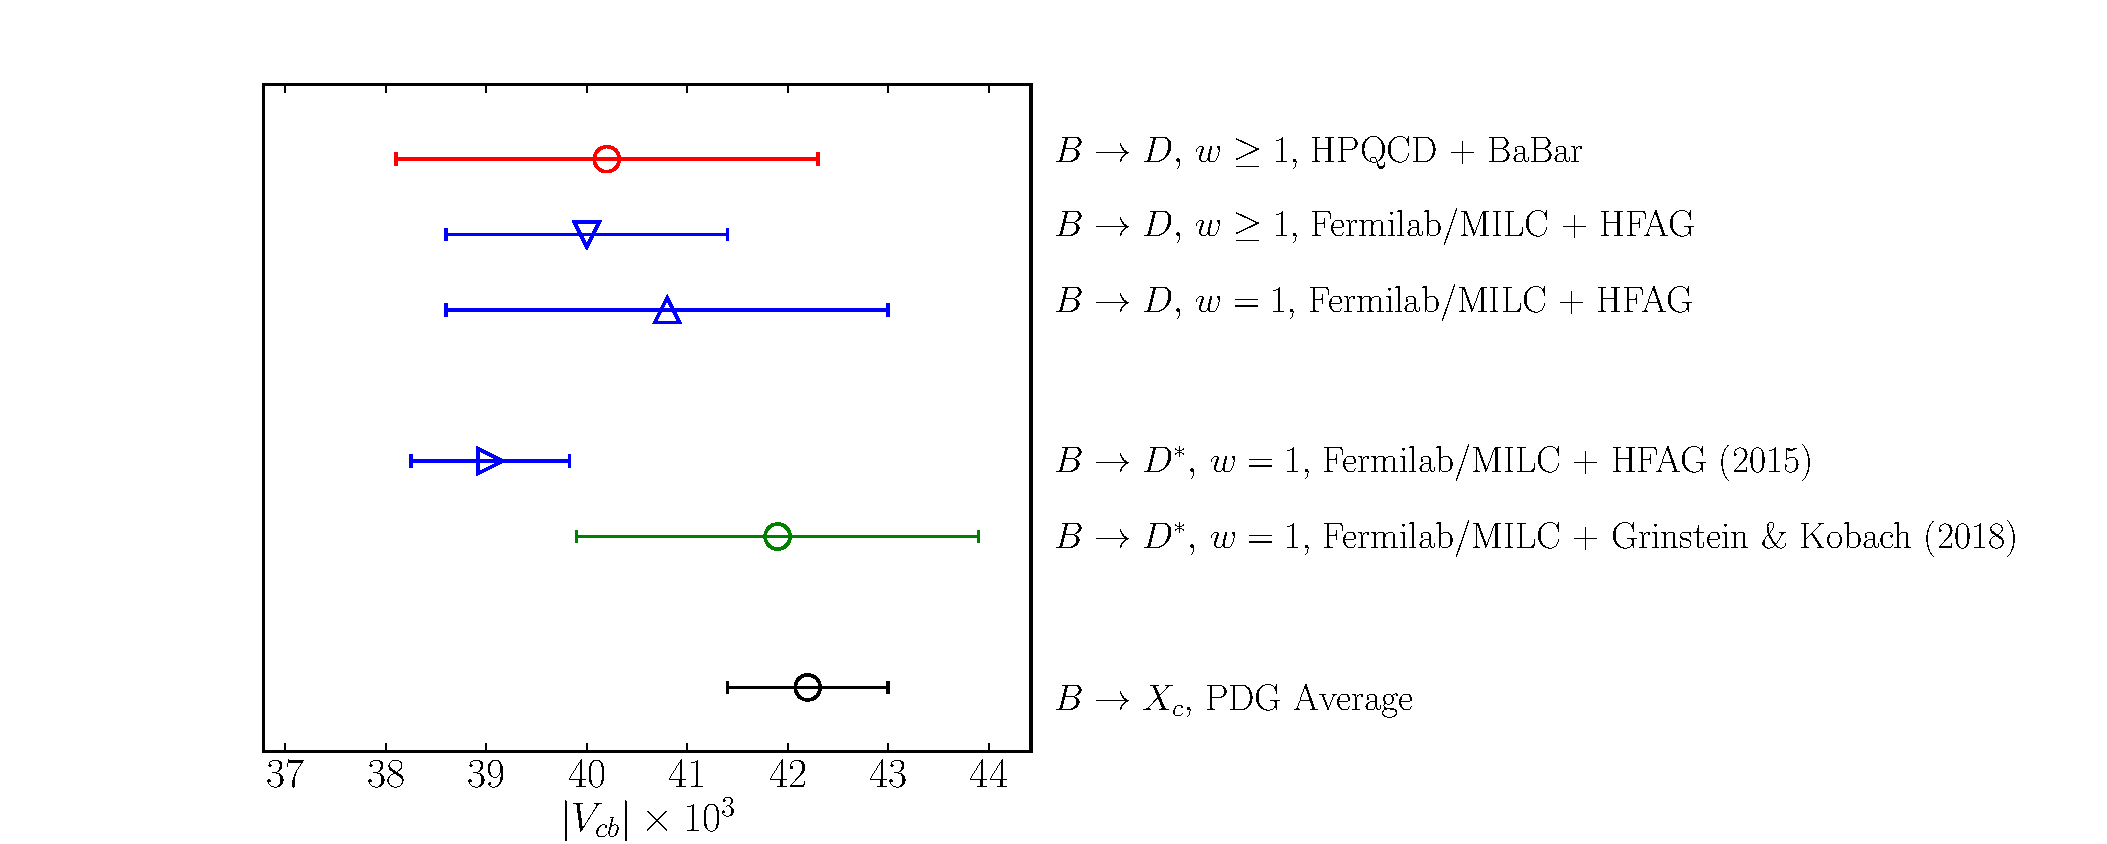
\includegraphics[width=1.2\textwidth]{images/Vcb_plot.pdf}
%  \end{center}
%  \vspace{-20pt}
  \caption{Different determinations of $|V_{cb}|$. Points labelled $w=1$ are determinations from extrapolating measurements of decay rates to the zero recoil point and combining them with a lattice determination of the form factor at zero recoil. Points labelled $w\geq 1$ are results from using a combination of both branching fractions and lattice form factors through some range of $w$. The first name mentioned in the labels give the source of the lattice form factors, and the second gives the source of the experimental data (e.g. the HPQCD$+$BaBar point used form factors from the HPQCD collaboration and data from the BaBar experiment). The highest point in red is from \cite{Na:2015kha}, the second and third highest from \cite{Lattice:2015rga}, fourth from \cite{Bailey:2014tva}, fifth from \cite{Grinstein:2017nlq}. The bottom point is from the PDG \cite{PhysRevD.98.030001}, using data from the ALPEPH \cite{BUSKULIC1995236}, Belle \cite{Abe:2001yf}, BaBar \cite{Aubert:2008yv,Aubert:2009ac}, and CLEO \cite{Bartelt:1998dq} experiments.
    \label{fig:Vcb_plot}}
\end{figure}

This figure tells a story of the recent history of $|V_{cb}|$. Determinations from $B\to D\ell\nu$ have been consistent with, but not as precise as, the other two methods. Until recently, there was a $\sim3\sigma$ tension between determinations from the $B\to D^* \ell\nu$ decay and inclusive decays. A possible explaination of this tension appeared when concern was raised about the method of extrapolating experimental data for $B\to D^*l\bar{\nu}$ decay rates to the zero recoil point ($w=1$) \cite{Bernlochner:2017jka, Bigi:2017njr, Grinstein:2017nlq}..

The Heavy Flavor Averaging Group HFAG (Now HFLAV) determination of $|V_{cb}h_{A_1}(1)|$ in 2015 parameterized the form factors in the extrapolation using the CLN parameterisation \cite{Caprini:1997mu}. It has become clear that the constraints imposed on the form factors in the CLN parameterisation are not justified. In \cite{Bigi:2017njr,Grinstein:2017nlq}, the results of an extrapolation using the CLN parameterisation were compared to results from a more general, model-independent parameterisation, the BGL parameterisation \cite{GLENNBOYD1996493}. It was found that they differed by $3.5\sigma$. Since BGL is model independent, one may consider this the more reliable result.

The $|V_{cb}|$ result using BGL to extrapolate the decay rates is given in the green point on Fig. \ref{fig:Vcb_plot}. Hence, if this work is to be trusted, the long-standing $|V_{cb}|$ tension has been resolved.

There are however a number of other reasons to be interested in studying $|V_{cb}|$. It constrains one side of the unitarity triangle via the ratio $|V_{ub}|/|V_{cb}|$, so it is one of the bottlenecks for precise tests of CKM unitarity. It is also a dominant uncertainty in the determination of the $CP$-violation parameter $\epsilon_K$ (that is currently at tension between the SM and experiment, see for example \cite{Bailey:2018feb} where a $4\sigma$ tension is reported).

%% A dominant motivation for the work presented in this thesis is the quest for a more precise determination of $|V_{cb}|$. The main results are form factors for $B_s\to D_s l\bar{\nu}$ and $B_s\to D_s^* l\bar{\nu}$. The benefit of these determinations is two-fold. Firstly, they can be combined with future experimental measurements of $B_s\to D_s^{(*)}l\bar{\nu}$ decays for a new $|V_{cb}|$ determination. Increasing the number of independent determinations of $|V_{cb}|$ makes each result more robust. Secondly, they demonstrate that our approach in the lattice calculations work well and can, therefore, be applied to $B\to Dl\bar{\nu}$ and $B\to Dl\bar{\nu}$ form factors in the future.

\subsection{Flavor Anomalies \& Lepton Flavor Violation}

The SM can be tested by studying semileptonic decays more directly, without any consideration of CKM elements. CKM-independent observables can be constructed by taking ratios of branching fractions for decays with common CKM dependence. Then, form factors from lattice QCD can be used to form pure SM predictions of these ratios and compared to purely experimental measurements. Such comparisons have uncovered a number of tensions between the SM and experiment.

The ratios are defined by
\begin{align}
  R_{X_q} = {\Gamma(B_q\to X_q \tau \nu_{\tau}) \over {1\over 2}\left[\Gamma(B_q\to X_q e \nu_e) + \Gamma(B_q\to X_q \mu \nu_{\mu}) \right]},
  \label{eq:Rratios}
\end{align}
where $X_q$ is any meson with valence quark content of $x\bar{q}$. The numerator and denomenator will have a common factor of $|V_{bx}|$, so cancel in the ratio.

There is currently tension between SM and experiment in $R_D$ and $R_{D^*}$:
\begin{gather}
  R_{D^*}|_{\text{exp}} = 0.306(13)_{\text{stat}}(07)_{\text{sys}}\,,\quad\,\,\, R_{D^*}|_{\text{SM}} = 0.258(5),
  \\
  R_D|_{\text{exp}} = 0.407(39)_{\text{stat}}(24)_{\text{sys}}\,,\quad\quad R_D|_{\text{SM}} = 0.299(3).
\end{gather}
The expermental values are the HFLAV averages, from BaBar \cite{Lees:2012xj,Lees:2013uzd}, Belle \cite{Huschle:2015rga,Sato:2016svk,Hirose:2016wfn,Hirose:2017dxl}, and LHCb \cite{Aaij:2015yra,Aaij:2017uff,Aaij:2017deq} data. 
The value for $R_{D^*}|_{\text{SM}}$ is the average of results from \cite{Bigi:2016mdz,Bernlochner:2017jka,Jaiswal:2017rve}, using a combination of light-cone sum rules and form factor constraints due to heavy quark symmetry. The $R_{D}|_{\text{SM}}$ value is the average of results from \cite{Bernlochner:2017jka,Bigi:2017jbd,Jaiswal:2017rve}, which used lattice form factors from \cite{Na:2015kha,Lattice:2015rga}.

A joint analysis of $R_D$ and $R_{D^*}$ by HFLAV shows the combined tension to have a significance of $4.0\sigma$ (see Fig. \ref{fig:ratiotension}). Clearly more precise experimental results are necessary to either confirm or dismiss this anomaly. While the SM values are currently much more precise than the experimental ones, further work on the theoretical results is necessary. More independent calculations are required to make the SM numbers more robust, such that if this tension ever hits $5\sigma$, we can be confident that it is due to new physics and not some underestimated SM systematic.

\begin{figure}
  \begin{center}
    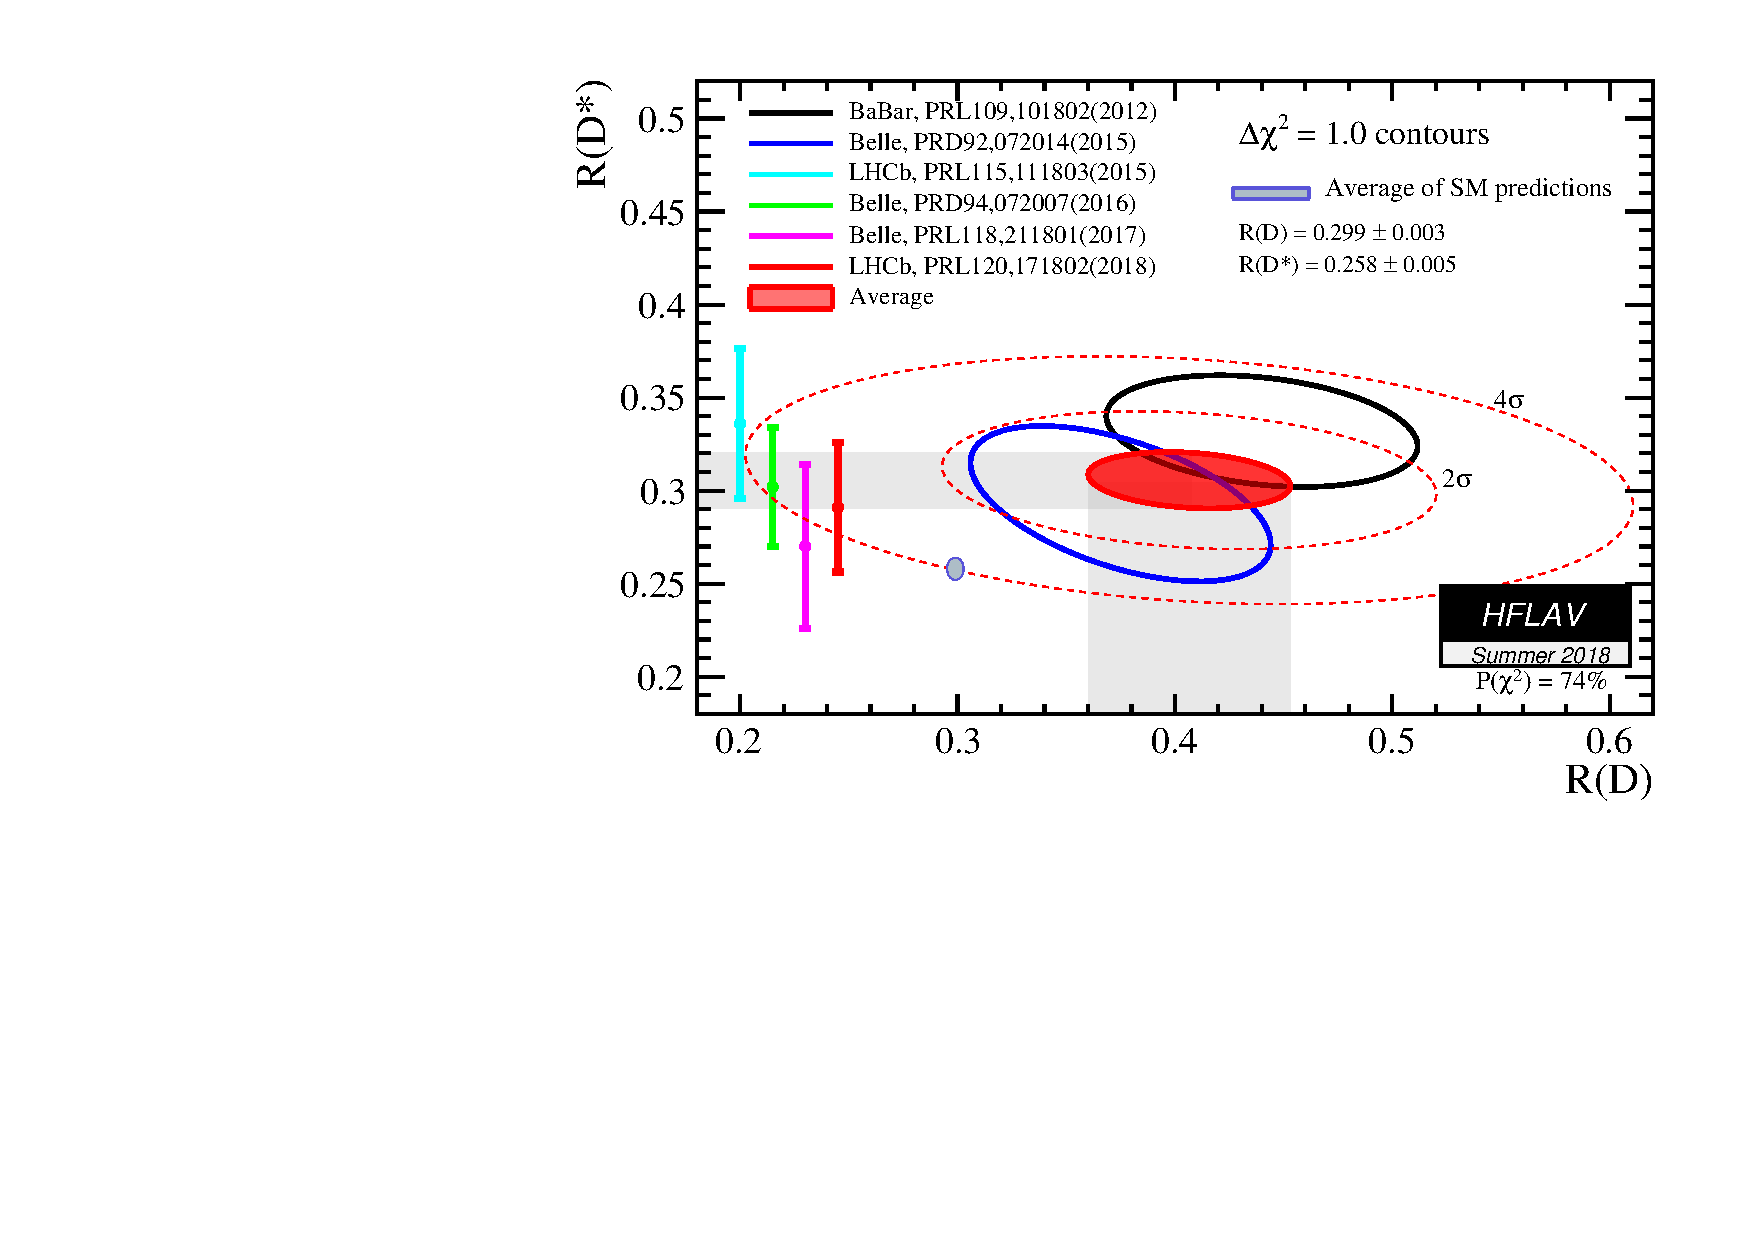
\includegraphics[width=
      0.8\textwidth]{images/rdrds_summer18.pdf}
  \end{center}
  \caption{$R(D^{(*)})$ determinations from SM and measurement
    \cite{HFLAV16}. One can see from this that the SM prediction (the small blue ellipse) is inconsistent with the experimental average (the filled red ellipse).
    \label{fig:ratiotension}}
\end{figure}

There are also tensions in the quantitites \cite{Altmannshofer:2017yso}
\begin{align}
  R_{K^{(*)}} = {\Gamma( B\to K^{(*)}\mu^+\mu^-)\over \Gamma( B\to K^{(*)} e^+e^-)}.
\end{align}
LHCb measured $R_K$ between 1 and 6GeV, and found a disagreement with the SM value \cite{Bobeth:2007dw,Bouchard:2013mia} of 2.6$\sigma$ \cite{Aaij:2014ora}. LHCb also measured $R_{K^*}$ in 2 bins ($0.045<q^2<1.1 $GeV$^2$ and $1.1<q^2<1.6$GeV$^2$), and reported disagreement with the SM prediction \cite{Bordone:2016gaq,Descotes-Genon:2015uva,Capdevila:2016ivx,Capdevila:2017ert,Serra:2016ivr,Straub:2015ica,Altmannshofer:2017fio,Jager:2014rwa} of 2.1-2.3$\sigma$ and 2.4-2.5$\sigma$ respectively \cite{Aaij:2017vbb}.

%% A useful direction we could go in, besides improving the precision of these ratios, is to test other ratios where LFV should show up. For example, in this thesis, we provide a new prediction of $R_{D_s}$, which when combined with future experimental data, will help clarify this picture.

Each of these anomalies points to one potential new physics scenario: lepton flavor violation (LFV). This is a breakdown of the lepton flavor universality in the SM discussed earlier in this section. A consequence of LFV would be that the different lepton generations would no longer have the same coupling to gauge fields. For example, imagine couplings like $U_{ij} \bar{e}_L^i \slashed{W}^+ \nu_L^j$, where $U_{ij}$ is unitary but non-diagonal, then the different lepton generations would have different couplings to $W$. This can lead to a modification of the $B\to D^{(*)}\ell\nu$ and $B\to K^{(*)}\bar{l}l$ decays rates by different amounts depending on the lepton flavors in the final state, resulting in the ratios $R_{D^{(*)}}$, $R_{K^{(*)}}$ deviating from the SM prediction.

There are broadly speaking two ways one can explain LFV. The first is to posit that there are in fact right-handed neutrinos, $\nu_R$, and neutrinos have Dirac mass terms $m\bar{\nu}_L\nu_R$ (from a coupling to the Higgs). Then, the argument preventing the presence of non-trivial lepton flavor structure in $\mathcal{L}_{\text{FCCC}}$ breaks down, we obtain an equivalent of the CKM matrix for leptons (the Pontecorvo-Maki-Nakagawa-Sakata (PMNS) matrix). Lepton flavor violation is then mediated by the $W$. Neutrinos have in fact already been shown to have mass, the PMNS matrix exists, and its elements have been measured. However, as mentioned already, these effects would be extremely small due to the extremely small mass of the neutrinos. Experiments have looked for evidence of $W$-mediated LFV processes, $\tau\to \mu\gamma$ and $\mu\to e\gamma$, and they found upper bounds for their branching fractions of $4.2\times 10^{-13}$ \cite{Abe:2003sx} and $3.1\times 10^{-7}$ \cite{TheMEG:2016wtm} respectively.

Besides there being no evidence for $W$-mediated LFV, this picture of neutrino masses is not very aesthetically satisfying. It requires unnaturally small Yukawa couplings between the Higgs and the neutrinos. The second,  much more popular approach to explaining both LFV and neutrino masses is the existence of new particles.

In the face of evidence against the SM, the most general way to parameterise the space of possible new physics models is to study the Standard Model Effective Theory (SMEFT) \cite{Brivio:2017vri}. In this approach, one introduces higher dimension, non-renormalisable operators to the SM (the SM has only dimension 4 operators), and impose a hard momentum cutoff $\Lambda$. Then the SMEFT is
\begin{align}
  \mathcal{L}_{\text{SMEFT}} = \mathcal{L}_{\text{SM}} + \sum_i {c^{(5)}_i\over\Lambda} \mathcal{O}^{(5)}_i + \sum_i {c^{(6)}_i\over\Lambda^2} \mathcal{O}^{(6)}_i + ...
\end{align}
where $\{\mathcal{O}_i^{(d)}\}$ is the set of dimension-$d$ operators that satisfy the symmetries of the SM, and $\{c_i^{(d)}\}$ are coefficients to be measured, known as Wilson coefficients. Wilson coefficients differing from the SM expectation can be evidence that the SM must be augmented with new fields at energies above $\Lambda$. The quantum numbers of the associated operators gives information about the quantum numbers of the new fields.

One can fit the avaliable $B\to D^{(*)}l\bar{\nu}$ and $B\to K^{(*)}\bar{l}l$ data to predictions from SMEFT, in order to infer the Wilson coefficients neccesary to explain the anomalies. In \cite{Freytsis:2015qca} it was found that $R_{D^{(*)}}$ can be explained with the $d=6$ operators:
\begin{gather}
  \nonumber
  (\bar{c}\gamma_{\mu}P_L b)(\bar{\tau}\gamma^{\mu} P_L \nu_{\tau}), \quad
  (\bar{c}\sigma^{\mu\nu} P_L b)(\bar{\tau} \sigma_{\mu\nu} P_L \nu_{\tau}), \quad
  (\bar{\tau} P_L c^c)(\bar{b}^c P_L \nu_{\tau}), \\
  (\bar{\tau}\gamma_{\mu} P_R b) (\bar{c} \gamma^{\mu} P_L \nu_{\tau}), \quad
  (\bar{\tau}\gamma_{\mu}P_L b)(\bar{c}\gamma^{\mu} P_L \nu_{\tau}), \quad
  (\bar{\tau}P_R c^c)(\bar{b}^c \gamma^{\mu} P_L \nu),
\end{gather}
where $P_{L/R} = (1\pm \gamma_5)/2$, $\psi^c = -i(\bar{\psi}\gamma^0\gamma^2)^T$ and $\bar{\psi}^c = -i(\gamma^0\gamma^2 \psi)^T$. In \cite{Altmannshofer:2017yso}, a similar process found the operators neccesary to explain $R_{K^{(*)}}$:
\begin{gather}
  \nonumber
  (\bar{s}\gamma_{\mu}P_L b)(\bar{e}\gamma^{\mu}e), \quad (\bar{s}\gamma_{\mu}P_L b)(\bar{\mu}\gamma^{\mu}\mu) \\
  (\bar{s}\gamma_{\mu}P_L b)(\bar{e}\gamma^{\mu}\gamma_5e), \quad (\bar{s}\gamma_{\mu}P_L b)(\bar{\mu}\gamma^{\mu}\gamma_5\mu)
\end{gather}
This information, along with constraints from other measurements, strongly reduces the space of possible new physics models that could produce these anomalies. Hot topics include Leptoquarks, $Z'$ models, and partial compositeness \cite{Altmannshofer:2017yso,Freytsis:2015qca,Bauer:2015knc,Crivellin:2015mga}.



%%%%%%%%%%%%%%%%%%

\section{Strong Interaction Physics}
\label{sec:stronginteractions}

The work of this thesis is essentially quantifying the effect that the strong interaction has on branching fractions for semileptonic decays. The strong interaction and the observed pattern of hadrons can be explained with QCD. In this section, I review the fundamental theory and the force's physical features.

\subsection{Quantum Chromodynamics}
\label{sec:qcd}

QCD is an $SU(3)$ Yang-Mills gauge theory. The Lagrangian is derived by requiring:
\begin{itemize}
\item
  $N_f$ fermion fields transforming in the fundamental representation of the $SU(3)$ gauge group.
\item
  Invariance under that gauge group.
\item
  Renormalizability of all interactions.
\end{itemize}
From these we find \cite{Schwartz:2013pla}:
\begin{align}
    \label{eq:qcdlag}
  \mathscr{L}_{\text{QCD}} &= \sum_i \bar{q}_i (i \slashed{D} - m_i) q_i - {1\over 4} \text{Tr}G_{\mu\nu} G^{\mu\nu} - g{\bar{\theta}\over 64 \pi^2} \epsilon^{\mu\nu\rho\sigma} \text{Tr}G_{\mu\nu} G_{\rho\sigma} \\
  &D_{\mu} = \partial_{\mu} - i g G_{\mu} \,,\quad
  G_{\mu\nu} = [ D_{\mu}, D_{\nu} ].
  \nonumber
\end{align}
$q_i = ( q_{i,r}, q_{i,b}, q_{i,g} )$ are the $N_f$ fermions, vectors in {\it{color space}}, transforming under
\begin{align}
  q_i(x) \to \Lambda(x)q_i(x) \,,\, \bar{q}_i(x) \to \bar{q}_i(x) \Lambda^{\dagger}(x),
  \label{eq:quark_gauge_trans}
\end{align}
where $\Lambda(x)$ is an $SU(3)$ matrix acting on the color space. $G_{\mu}$ are the $\mathfrak{su}(3)$-valued gluon fields, transforming under the gauge group like
\begin{align}
  G_{\mu}(x) \to \Lambda(x) G_{\mu}(x) \Lambda^{\dagger}(x) - {i\over g} [ \partial_{\mu} \Lambda(x) ] \Lambda^{\dagger}(x).
  \label{eq:G_gauge_trans}
\end{align}
$g$ is the coupling constant of the theory, often expressed instead as $\alpha_s = (g/4\pi)^2$. $\bar{\theta}$ has strong experimental bounds on its size, to the extent that for our purposes that term can be neglected \cite{ALTAREV1992242}.

The most notable feature of QCD is due to the running of $\alpha_s$ \cite{PhysRevLett.30.1343}.
\begin{figure}
  \begin{center}
    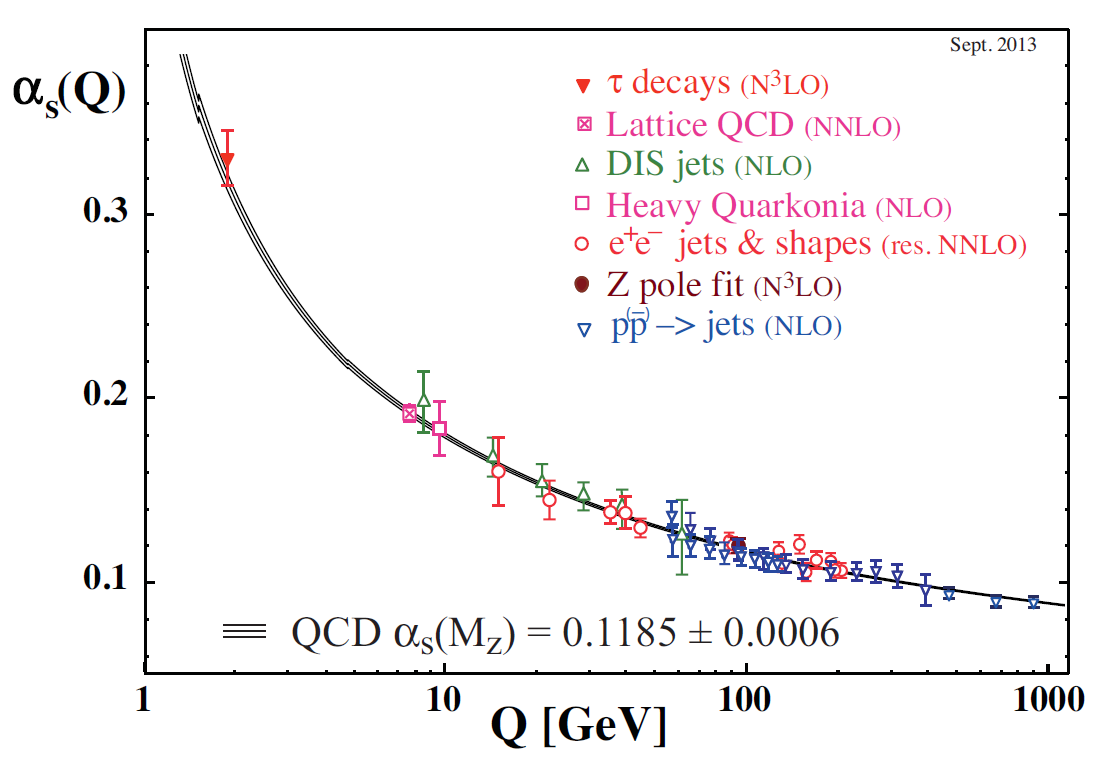
\includegraphics[width=0.7\textwidth]{images/QCD-running-coupling.png}
  \end{center}
  \caption{The relationship between scale $Q$ and the strong coupling constant $\alpha_s$, from the PDG \cite{PhysRevD.98.030001}.}
  \label{fig:alpha_s}
\end{figure}
Unlike in quantum electrodynamics where the coupling increases with energy scale, the coupling of QCD decreases as energy scales increase. This is referred to as {\it{asymptotic freedom}}. A corollary is that at low energies the coupling becomes strong. At energies around or below $\Lqcd \sim 0.5$GeV, $\alpha_s$ becomes too large to be a good expansion parameter, and perturbation theory becomes unreliable for making predictions.

At large $\alpha_s$, quarks and gluons become strongly interacting. This is believed to be the source of confinement, the mechanism that binds quarks together into hadrons. %A common assumption then is that all of the dynamics that occur inside hadrons have energies on the scale of $\Lqcd$.

Broadly speaking there are two approaches to making predictions in QCD at low energies:
\begin{enumerate}
\item
  Chiral perturbation theory - an effective theory of hadrons with the same symmetry properties as QCD.
\item
  Lattice QCD calculations - solve the path integral by brute force, eliminating the need for an expansion in $\alpha_s$. This is covered in chapters \ref{chap:latticeqcd} and \ref{chap:latticecalculations}.
\end{enumerate}

\subsection{Chiral Symmetry}
\label{sec:chiralsymmetry}

Here I follow the discussion in \cite{Scherer:2002tk}. In the limit of $m_i\to 0\,\,\forall i$, QCD develops two new global symmetries between the flavors:
\begin{align}
  \label{eq:vector_chiral}
  q_i &\to \exp(i\theta_a^V \lambda^{ij}_a) q_j\,, \\
  q_i &\to \exp(i\gamma_5 \theta_a^A \lambda^{ij}_a) q_j\,,
\end{align}
where $\lambda_a$ are $U(N_f)$ generators. They are labelled $U(N_f)_V$ and $U(N_f)_A$ respectively, standing for vector and axial-vector.
% Each of these groups can be decomposed into $U(1)_{V/A}\times SU(N_f)_{V/A}$, the $U(1)$ contains the single element corresponding to $\lambda_a=1$, and $SU(N_f)$ contains the elements where $\lambda_a$ are $SU(N_f)$ generators. Neccesary?

From Noether's theorem, each generator of these symmetries implies a current that is conserved in the massless limit:
\begin{align}
  \label{eq:chiralcurrents}
  V_{\mu}^a = \bar{q} \gamma_{\mu} \lambda_a q\,, \quad\quad
  A_{\mu}^a = \bar{q} \gamma_{\mu} \gamma_5 \lambda_a q\,.
\end{align}

The (partial) conservation of these currents in quantum mechanics is captured by the {\it{Ward identities}}. There is an infinite number of possible Ward identities, but for the purpose of this work, we only need to consider the most simple of them. %We will derive these below.

Consider the partition function for QCD:
\begin{align}
  \mathcal{Z} = \int [d\psi d\bar{\psi} dA] e^{iS[\psi,\bar{\psi},A]},
\end{align}
where $[d\psi d\bar{\psi} dA]$ represents the functional integral over quark, antiquark and gauge fields. Consider performing a shift of the integration variables of the form \eqref{eq:vector_chiral}, and allow the parameters $\theta_a$ to be local, $\theta_a=\theta_a(x)$. The partition function becomes
\begin{align}
  \mathcal{Z} = \int \mathcal{J} [d\psi d\bar{\psi} dA] ( 1 + i\delta S ) e^{iS[\psi,\bar{\psi},A]}\,.
  \label{eq:partition_transformed}
\end{align}
%$\mathcal{J}$ is the Jacobian of the measure $[d\psi d\bar{\psi} dA]$ under the coordinate transform \eqref{eq:vector_chiral}. In many cases, this will be non-trivial, even if the transform is classically a symmetry of the theory. This can be due to a regularization of the path integral that does not respect the symmetries of the theory. Alternatively, it could be due to an anomaly - an instance of a classical symmetry not holding in quantum mechanics. The symmetries we will be concerned with in this work will always be anomaly-free, so let's set $\mathcal{J}=1$.

$\mathcal{J}$ is the Jacobian of the measure $[d\psi d\bar{\psi} dA]$ under the coordinate transform \eqref{eq:vector_chiral}. In many cases, $\mathcal{J}$ will be non-trivial, due to either regularization schemes that don't respect the symmetry or quantum anomalies. The symmetries we are concerned with here are anomaly free, so $\mathcal{J}=1$.

The effect of the local version of Eq. \eqref{eq:vector_chiral} on the action is
\begin{align}
  \delta S = \int d^4x \theta_a(x) \left[ \partial_{\mu} V_a^{\mu}(x) - i\bar{q}(x) [\lambda_a,M] q(x) \right],
\end{align}
where $M = \text{diag}(m_u,m_d,m_s,...)$ acts on flavor. Removing $\mathcal{Z}$ from each side of \eqref{eq:partition_transformed}, setting the arbitrary functions $\theta_a(x)$ to $1$, and removing the spacetime integral results in
\begin{align}
  \partial_{\mu}\langle V_a^{\mu} \rangle = i \langle \, \bar{q} [ \lambda_a, M ] q \, \rangle,
  \label{eq:vector_ward}
\end{align}
where $\langle \rangle$ represents a quantum expectation value, the state the expectation value is taken in need not be specified since the above derivation does not assume any particular state. Repeating the above steps with the vector chiral transform replaced with the axial-vector chiral transform, one finds
\begin{align}
  \partial_{\mu}\langle A_a^{\mu} \rangle = i \langle\, \bar{q} \{ \lambda_a,M \} q \,\rangle.
  \label{eq:axial_ward}
\end{align}
\eqref{eq:vector_ward} and \eqref{eq:axial_ward} are examples of Ward identities, they describe the (parital) conservation of the chiral currents. \eqref{eq:vector_ward} is often referred to as the Partially Conserved Vector Current (PCVC) relation, and \eqref{eq:axial_ward} the Partially Conserved Axial Current (PCAC) relation.

A useful theorem \cite{Fubini:1964boa} is that partially conserved currents (currents that become conserved when some parameter in the theory vanishes, like $V^{\mu}_a$ and $A^{\mu}_a$) require no renormalisation in any regularisation scheme. %We will now demonstrate this.
The conserved or partially conserved current $J_a^{\mu}$ has a corresponding charge $Q_a(t) = \int d^3x J_a^{0}(\underline{x},t)$ that is the generator of its corresponding symmetry transform on Hilbert space. In this case, these charges are members of the Lie algebra of the symmetry group:
\begin{align}
  [ Q_a(t), Q_b(t) ] = if_{abc} Q_c(t)\,,
  \label{eq:charge_commutator}
\end{align}
where $f_{abc}$ are the structure constants of the algebra. Under some regularization, change in regularization scheme, or running of scale, each operator in the theory may require multiplicative renormalization $Q_a \to Z_Q Q_a$. Eq. \eqref{eq:charge_commutator} demands that $Z_Q=1$ in all cases. So $J^0$ obtains no renormalisation, and if the regularization is Lorentz invariant, this carries on to $J^{\mu}$.

%% In the case of the chiral currents $V_a^{\mu},A_a^{\mu}$, the Ward identities \eqref{eq:vector_ward}, \eqref{eq:axial_ward} cause this property to carry onto the operators on the LHS, $\bar{q} [\lambda_a,M] q$ and $\bar{q} \{ \lambda_a,M \} q$, these operators receive no normalisation under any regularisation scheme.

Since one can transform any flavor into any other flavor via the chiral $U(N_f)$ generators, one can build currents charged with any combination of flavors from linear combinations of $V_a^{\mu}$ and $A_a^{\mu}$:
\begin{align}
  \label{eq:vector_ward_indiv}
  V_{ij}^{\mu} &= \bar{q}_i \gamma^{\mu} q_j \,,\quad\quad \partial_{\mu}\langle V^{\mu}_{ij} \rangle = i ( m_i - m_j ) \langle S_{ij} \rangle \\
  A_{ij}^{\mu} &= \bar{q}_i \gamma^{\mu}\gamma^5 q_j \,,\quad \partial_{\mu}\langle A^{\mu}_{ij} \rangle = i ( m_i + m_j ) \langle P_{ij} \rangle
  \label{eq:axial_ward_indiv}
\end{align}
where we have defined $S_{ij} = \bar{q}_iq_j$ and $P_{ij} = \bar{q}_i\gamma^5 q_j$, the scalar and pseudoscalar densities. The non-renormalisation of $V_a^{\mu}$ and $A_a^{\mu}$ carry on to $V_{ij}^{\mu}$ and $A_{ij}^{\mu}$, and onto the operators $( m_i - m_j ) S_{ij}$, $( m_i + m_j ) P_{ij}$ via the Ward identities.

The partially conserved currents $V^{ij}_{\mu}$ and $A^{ij}_{\mu}$ are the same currents that feature in the matrix element of leptonic and semileptonic decays in Sec. \ref{sec:fccc}, and their expectation values appear in amplitudes for leptonic and semileptonic decays. Hence, the fact that these can be related to alternative expectation values via ward identities, and that they obtain no renormalisation, is very useful in the calculation of these amplitudes.

\section{Heavy Quark Physics}

Quarks with mass $m_Q \gg \Lqcd$ are referred to as heavy quarks. Charm and bottom quarks are considered heavy: $\Lqcd/m_c \sim 1/4$, $\Lqcd/m_b \sim 1/14$. This separation of scales can come in very useful. They mean one can integrate out some degrees of freedom at $m_Q$, and still have a good description of the dynamics at $\Lqcd$. This philosophy gives rise to Heavy Quark Effective Theory (HQET) and Non-Relativistic QCD (NRQCD). Below I will summarise the aspects of this theory most relevant to our work.

%% The physical picture of a meson containing a heavy quark is very similar to that of a hydrogen atom. In the hydrogen atom, the nucleus has a mass much greater than the characteristic energies of the electron and photons. One can treat the nucleus as a static source of electric charge, and solve to high precision the dynamics of the electron. The electron's behaviour is not affected by the mass or the spin of the nucleus. Similarly, one can consider a heavy quark in a meson to be a static source of colour charge, and solve the $\Lqcd$ dynamics in its presence. The mass and spin of the heavy quark does not effect the light degrees of freedom, this is the well understood {\it{heavy quark symmetries}}. The effective field theories introduced in this section gives us a framework to take this approximation and systematically correct for it.

\subsection{HQET}

HQET \cite{Georgi:1990um} is an effective field theory with the cutoff at the heavy quark mass $m_Q$, and operators organized in a series in $\Lambda_{\text{QCD}}/m_Q$. Since at the $b$ (and $c$) mass QCD is perturbative ($\alpha_s(m_Q) \ll 1$), one can match HQET to perturbative QCD at $m_Q$, then run the couplings of HQET down to produce useful predictions at the confinement scale.

%% It is a useful tool for when we perform extrapolations in heavy quark mass, as it supplies us with explicit expressions for the heavy quark mass dependence on various phenomenological quantities.

\subsubsection{HQET Lagrangian}

Here is the derivation of HQET for a single heavy quark interacting with gluons, following \cite{Neubert:2005mu} (the generalization to many flavors is straightforward). The fermion part of the Lagrangian is
\begin{align}
  \mathscr{L}_{\text{QCD}} = \bar{Q} ( i\slashed{D} - m_Q ) Q\,,
  \label{eq:dirac}
\end{align}
where $Q$ is the heavy quark field and $D$ is the covariant derivative (Eq. \eqref{eq:qcdlag}). Define the heavy quark velocity $v$ according to $v = p_Q/m_Q$. Split $Q$ into ``heavy'' ($H$) and ``light'' ($h$) components:
\begin{align}
  \label{eq:hdef}
  Q = e^{im_Q v\cdot x}(h + H)\quad : \quad &h = {1\over 2} e^{-im_Q v\cdot x} ( 1 + \slashed{v} ) Q, \\
  &H = {1\over 2} e^{-im_Q v\cdot x} ( 1 - \slashed{v} ) Q\,,
\end{align}
with the important property
\begin{align}
  \slashed{v} h = h \quad \slashed{v} H = - H.
\end{align}
In terms of these new fields the Lagrangian becomes
\begin{align}
  \mathscr{L}_{\text{QCD}} = i\bar{h} (v\cdot D) h - \bar{H} ( i(v\cdot D) + 2m_Q ) H
  + i \bar{h} \slashed{D}^{\perp} H + i \bar{H} \slashed{D}^{\perp} h\,,
  \label{eq:HQET_preintegral}
\end{align}
where $D^{\perp} = D - v(v\cdot D)$ are the components of $D$ perpendicular to $v$. %In the rest frame of the heavy quark, $v = (1,0,0,0)$ so $v_{\mu}(v\cdot D)$ becomes the temporal derivative and $D^{\perp}$ the spatial.
A physical interpretation of the definition of $h$ in Eq. \eqref{eq:hdef} can be seen by acting a spatial derivative on the definition of $h$, and by recognising $\partial Q = -i p_Q$, $\partial h = -i p_h$, we find that
\begin{align}
  p_Q = m_Q v + p_h.
\end{align}
Since $p_h \ll p_Q$, we see that the quark's momentum is dominated by its mass (the quark is close to on-shell), and the $h$ field represents perturbations around on-shell due to interactions with the lighter degrees of freedom at $\Lambda_{\text{QCD}}$.

From the Lagrangian \eqref{eq:HQET_preintegral}, we see that $h$ is a massless field and $H$ has a mass of $2m_Q$. From this Lagrangian we can derive an equation of motion for $H$:
\begin{align}
  ( i(v\cdot D) + 2m_Q) H = i\slashed{D}^{\perp} h,
\end{align}
with the solution
\begin{align}
  H = {1\over i(v\cdot D) + 2m_Q} i\slashed{D}^{\perp} h = {1\over 2m_Q}\sum_{n=0}^{\infty} {(-i(v\cdot D))^n\over 2m_Q} \slashed{D}^{\perp} h.
\end{align}
By substituting this into the Lagrangian \eqref{eq:HQET_preintegral} we arrive at
\begin{align}
  \mathscr{L}_{\text{HQET}} = i \bar{h} (v\cdot D) h - \bar{h} \slashed{D}^{\perp} {1\over 2m_Q}\sum_{n=0}^{\infty} {(-i(v\cdot D))^n\over 2m_Q} \slashed{D}^{\perp} h.
  \label{eq:HQET_lagrangian}
\end{align}
%This can be found by a more rigorous proof by performing the Gaussian integration over the $H$ field in the path integral {\color{red}{ref!}}.
Since we expect $v\cdot D \sim \Lambda_{\text{QCD}}$, we can interpret the infinite sum as a series in $\Lambda_{QCD}/m_Q$, and truncate it at some order. %For example to $\mathcal{O}(\Lambda_{\text{QCD}}/m_Q)$, we have
%% \begin{align}
%% \mathcal{L}_{\text{HQET}^1} = i \bar{h} (v\cdot D) h - {1\over 2m_Q} \bar{h} \slashed{D}^{\perp 2} h
%% \label{eq:HQET1}
%% \end{align}

Leading order HQET exhibits new symmetries not present in full QCD, known as the heavy quark symmetries. Since $m_Q$ is not present in the leading order Lagrangian, there is a flavor symmetry - a set of $N$ heavy quarks with the same $v$ can be mixed via an $SU(N)$ symmetry. Similarly, due to the absence of spin-mixing matrices, a heavy quark has an $SU(2)$ spin symmetry. At leading order a heavy quark in a meson behaves like a static color charge, the dynamics at $\Lambda_{\text{QCD}}$ are not affected by its mass or spin.

I will now use HQET to derive a useful theorem used in our work, following the proof given in \cite{Lebed:1991sq}.

%% \subsubsection{Isgur-Wise Function}
%% \label{sec:isgurwise}

%% A consequence of heavy quark symmetry relevant to semileptonic decays are the Wigner-Eckart theorems. Consider a transition amplitude between two heavy pseudoscalar mesons:
%% \begin{align}
%%   \langle M(v) | \bar{h} \Gamma h | M(v') \rangle
%% \end{align}
%% The spin structure of $| M(v) \rangle$ is $\gamma_5 (1-\slashed{v})$, this can be shown with the following argument. The state can be generally written as $| M(v) \rangle = \int d^4x d^4y f(x,y) \bar{h}(x) \gamma_5 q(y) | \Omega \rangle$ where $q$ is the light valence quark and $|\Omega\rangle$ is the interacting vacuum. Using $\slashed{v} h = h$, this can be reexpressed as $| M(v) \rangle = \int d^4x d^4y f(x,y) \bar{h}(x) \gamma_5 (1-\slashed{v}) q(y) | \Omega \rangle /2$. %Then via the spin symmetry, one can always rotate the $h$ spin in the meson state such that it matches the spin of the current, i.e. $h_{\alpha} \bar{h}_{\beta} \to 1_{\alpha\beta} f(h,\bar{h})$.

%% The amplitude can be written as
%% \begin{align}
%% \langle M(v) | \bar{h} \Gamma h | M(v') \rangle = m_M \text{Tr}[ {1\over 2} \gamma_5 (1 - \slashed{v}) \Gamma {1\over 2} \gamma_5 (1 - \slashed{v'}) \mathcal{M}(v,v')]
%% \label{eq:wignereckart1}
%% \end{align}
%% where $\mathcal{M}(v,v')$ can be any gamma-matrix valued function. The $m_M$ factor comes from the relativistic normalisation of the states. A general spin decomposition of this is
%% \begin{align}
%% \mathcal{M}(v,v') = \xi_0(v\cdot v') + \slashed{v} \xi_1(v\cdot v') + \slashed{v'} \xi_2(v\cdot v') + \slashed{v}\slashed{v'} \xi_4(v\cdot v').
%% \end{align}
%% Plugging this into \eqref{eq:wignereckart1}, we can then write the amplitude in terms of a single function:
%% \begin{align}
%% \langle M(v) | \bar{h} \Gamma h | M(v') \rangle = m_M \text{Tr}[ {1\over 2} \gamma_5 (1 - \slashed{v}) \Gamma {1\over 2} \gamma_5 (1 - \slashed{v'}) ] \xi(v\cdot v'),
%% \end{align}
%% where $\xi(v\cdot v') = \xi_0(v\cdot v') + \xi_1(v\cdot v') - \xi_3(v\cdot v') - \xi_4(v\cdot v')$ is known as the Isgur-Wise function. For a general pair of mesons with spin structure $\mathcal{H}$,$\mathcal{H}'$, a transition amplitude between them with a heavy current insertion can always be written as
%% \begin{align}
%% \langle \mathcal{H} | \bar{h} \Gamma h | \mathcal{H}' \rangle = \xi(v\cdot v') Tr[ \bar{\mathcal{H}} \Gamma \mathcal{H} ] + \order{\Lambda_{\text{QCD}}\over m_Q}
%% \end{align}
%% So all heavy semileptonic decays involving any combination of masses or spins are described by a single non-perturbative function, $\xi(v\cdot v')$. Examples relevant to the work of this thesis are:
%% \begin{align}
%% \langle D(v') | \bar{c_{v'}} \gamma^{\mu} b_v | B(v) \rangle &= \sqrt{m_B m_D} ( v + v')^{\mu} \xi(v\cdot v') \\
%% \langle D^*(v') | \bar{c_{v'}} \gamma^{\mu} b_v | B(v) \rangle &= i \sqrt{m_B m_D*} \epsilon^{\mu\nu\alpha\beta} \varepsilon_{\nu}^* v'_{\alpha} v_{\beta} \xi(v\cdot v')  \\
%% \langle D^*(v') | \bar{c_{v'}} \gamma^{\mu}\gamma_5 b_v | B(v) \rangle &= \sqrt{m_B m_D*} [ \varepsilon^{*\mu}(v\cdot v' + 1) - v^{'\mu} \varepsilon^*\cdot v] \xi(v\cdot v').
%% \end{align}
%% Here we have subscripted the fields $c_{v'}$,$b_v$ to specify the velocity used to separate those fields from the heavy components e.g. in eq. \eqref{eq:hdef}.

\subsubsection{Luke's Theorem}
\label{sec:Luke}

Luke's theorem \cite{LUKE1990447}, which can be derived from the Ademollo-Gatto (AG) theorem \cite{PhysRevLett.13.264}, tells us the leading order heavy quark mass dependence of form factors. First I will derive the AG theorem.

Consider the transition amplitude
\begin{align}
  \langle \alpha | Q_a | \beta \rangle,
\end{align}
where $Q_a$ is a conserved charge associated with some global symmetry $\mathcal{G}$, and $|\alpha\rangle$ and $|\beta\rangle$ belong to some irrep of $\mathcal{G}$, $\mathcal{R}(\mathcal{G})$. Imagine explicitly breaking the symmetry with a term like $\mathscr{L}_{\text{break}} = \lambda \mathcal{O}_{\text{break}}$. The states $|\alpha\rangle,|\beta\rangle$ are asymptotic states of the complete lagrangian including the symmetry breaking. The breaking causes the states to mix with states in other irreps of $\mathcal{G}$:
\begin{align}
  |\beta \rangle = c_{\beta\beta} | \beta' \rangle + \sum_{m} c_{\beta m} | m' \rangle \\
  \langle \alpha | = c^*_{\alpha\alpha} \langle \alpha' | + \sum_{n} c^*_{\alpha n} \langle n' |.
\end{align}
$|\alpha'\rangle,|\beta'\rangle$ are pure $\mathcal{R}(\mathcal{G})$ states, and $|m'\rangle,|n'\rangle$ are purely in some other irrep $\mathcal{R}'(\mathcal{G})$. The transition amplitude becomes
\begin{align}
  \nonumber
  \langle \alpha | Q_a | \beta \rangle
  =& c_{\alpha\alpha}^* c_{\beta\beta} \langle \alpha' | Q_a | \beta' \rangle \\
  \nonumber
  &+ \sum_m c_{\alpha\alpha}^* c_{\beta m} \langle \alpha' | Q_a | m' \rangle \\
  \nonumber
  &+ \sum_n c_{\alpha n}^* c_{\beta \beta} \langle n' | Q_a | \beta \rangle \\
  &+ \sum_m\sum_n c_{\alpha n}^* c_{\beta m} \langle n' | Q_a | m' \rangle.
  \label{eq:AGproofexpanded}
\end{align}
Since $|m'\rangle$ is purely in a different irrep to $|\alpha'\rangle$, $Q_a|m'\rangle$ has no overlap with $|\alpha'\rangle$. Similarly for $|n'\rangle$ and $|\beta\rangle$. Hence the second and third terms in Eq. \ref{eq:AGproofexpanded} vanish. Now consider the order of the coefficients $c_{nm}$. We can assume that $c_{nm} = \order{\lambda}$ for arbitrary $n,m \neq \alpha,\beta$, since switching off the symmetry breaking by setting $\lambda=0$ should cause $|\alpha\rangle $ and $|\alpha'\rangle$ to coencide. Then, using the normalization of the states $\sum_{n} |c_{\alpha n} |^2 = 1$, we find $c_{\alpha\alpha} = \sqrt{1 - \order{\lambda}^2} = 1 + \order{\lambda^2}$, and similarly for $c_{\beta\beta}$. Applying this to the two surviving terms in Eq. \eqref{eq:AGproofexpanded}, we end up with
\begin{align}
  \langle \alpha | Q_a | \beta \rangle = c + \order{\lambda^2},
\end{align}
where $c\neq c(\lambda)$. This is the AG theorem: if the current $Q_a$ and the symmetry breaking term $\mathcal{O}_{\text{break}}$ act orthogonally on the states, the transition amplitude can have at most a second order correction in the symmetry breaking parameter.

Now we can apply this to HQET to produce Luke's theorem. Consider a transition including two heavy quarks ($b$ and $c$). %% Then, the heavy quark symmetry is a spin symmetry for each flavor and a flavor symmetry between them. The leading order spin symmetry breaking terms can be found from Eq. \eqref{eq:HQET_lagrangian} to be
%% \begin{align}
%%   {1\over 4m_Q} \bar{h} \gamma^{\mu} \gamma^{\nu} G_{\mu\nu} h.
%% \end{align}
%% for both $h=b$ and $h=c$.
The theory is now HQET with two heavy quark flavors, $h=(b,c)$. Luke's theorem applies the AG theorem to the breaking of the flavor and spin symmetry at leading order HQET. First consider the flavor breaking. By unpacking the $1/m$-order terms in the Lagrangian \eqref{eq:HQET_lagrangian}, we find the leading order flavor breaking term to be
\begin{align}
  \left({1\over 2m_b} - {1\over 2m_c} \right) {1\over 2} \bar{h} \sigma_z \slashed{D}^{\perp 2} h,
\end{align}
where $\sigma_z$ is the third pauli matrix acting on flavor. These terms cause states like that of a $B$-meson, $| B \rangle$, to mix with other states $|n'\rangle$ in different irreps of the flavor symmetry. Consider for example the $B\to D$ decay at zero recoil. Since this is mediated by a generator of the flavor symmetry, the AG theorem leads to 
\begin{align}
  {\langle D | \bar{c}\gamma_{\mu} b | B \rangle \over \sqrt{M_B M_{D^*}}} &= \xi + \order{\left( {1\over 2m_b} - {1\over 2m_c} \right)^2}\,,
  \label{eq:B-D_lukestheorem}
\end{align}
where $\xi$ is some $b$- and $c$-mass independent number. This motivates a new parameterisation of pseudoscalar-pseudoscalar transition amplitudes alternative to \eqref{eq:formfactors_experimental}:
\begin{align}
  {\langle M' | V^{q_1q_2}_{\mu} | M \rangle \over \sqrt{Mm}} = h_+(w)(v+v')_{\mu} + h_-(w)(v-v')_{\mu}\,,
  \label{eq:pseudoscalar_hqet}
\end{align}
since Eq. \eqref{eq:B-D_lukestheorem} implies a form of $h_+(1)$ \cite{Falk:1992wt}:
\begin{align}
  h_+(1) &= \eta_V \left( 1 - l_P \left( {1\over 2m_b} - {1\over 2m_c} \right)^2 \right) + \mathcal{O}\left( \, {1\over m_c^n m_h^m}, \, n+m\geq 3 \, \right)\,.
  \label{eq:hplus}
\end{align}
$\eta_V$ is a matching factor between QCD and HQET, and can contain logarithms of heavy masses. The factor $l_P$ is a free non-perturbative parameter that must be fixed by some non-perturbative calculation e.g. a lattice QCD calculation.

Another decay that the AG theorem can be applied to is the $B\to D^*$ decay. At zero recoil, the amplitude of this decay is $\langle D^* | \bar{c} \gamma_{\mu}\gamma_5 b | B \rangle$. The operator here is not only a generator of the flavor symmetry but also of the spin symmetry, so we must also take spin breaking into account. The leading order spin breaking terms are
\begin{align}
  {1\over 2m_c} \bar{h}_c \gamma^{\mu} \gamma^{\nu} G_{\mu\nu} h_c + {1\over 2m_b} \bar{h}_b \gamma^{\mu} \gamma^{\nu} G_{\mu\nu} h_b\,.
\end{align}
So by an analagous argument to that of the $B\to D$ case, we end up with 
\begin{align}
  {\langle D^* | \bar{c}\gamma_{\mu}\gamma_5 b | B \rangle \over \sqrt{M_B M_{D^*}}} &= \xi + \order{\left( {1\over 2m_b} - {1\over 2m_c} \right)^2} + \order{\left({1\over 2m_c}\right)^2} + \order{\left({1\over 2m_b}\right)^2}\,.
\end{align}
This carries onto the form factor $h_{A_1}$ at zero recoil \cite{Falk:1992wt}:
\begin{align}
  \label{eq:hA1_hqet}
  h_{A_1}(1) =& \eta_A \left( 1 + {l_V\over (2m_c)^2} + {l_A\over 2m_b m_c} - {l_P\over (2m_b)^2} \right) \\ \nonumber
  & + \mathcal{O}\left( \, {1\over m_c^n m_h^m}, \, n+m\geq 3 \, \right)\,.
\end{align}
where $\eta_A$ is again a matching factor between HQET and QCD, and $l_{V,A,P}$ are non-perturbative quantities.


%% As we move away from the infinite-mass limit, $\xi$ becomes $h_+$, and $h_-$ becomes non-zero. In this case we see that
%% \begin{align}
%% h_+(q^2_{\text{max}}) &= ( 1 + \order{ \epsilon_b^2}
%% + \order{\epsilon_c^2} \\ &+ \order{\left( \epsilon_b - \epsilon_c \right)^2} ) \\
%% h_-(q^2_{\text{max}}) &= ( \order{ \epsilon_b }
%% + \order{ \epsilon_c } + \order{ \epsilon_b - \epsilon_c } )
%% \end{align}
%% Away from $q^2_{\text{max}}$, the velocities for the $b$ and $c$ quarks become different, resulting in a new flavor breaking term in the effective Lagrangian;
%% \begin{align}
%% i \bar{c} (v - v')\cdot D c \sim \order{1-{E_D\over M_D}} + \order{ \textbf{p}_D\over M_D }
%% \end{align}
%% where to deduce the orders we took the rest frame of the $B$ meson. This results in extra corrections of these orders (raised to the second power) in the form factors.

%% \subsubsection{Second Order Form Factors}

%% The process in \ref{sec:isgurwise} of decomposing matrix elements into general expressions parameterized by non-perturbative functions can be extended beyond leading order in HQET. In \cite{Falk:1992wt} this process was continued to second order in $1/m_b$ and $1/m_c$ for $B\to D^{(*)}$ transitions. The form factors for general $v,v'$ that are relevant to our work, were found to have the forms
%% \begin{align}
%% h_+ &= \xi + (\epsilon_b + \epsilon_c ) L_1 + ( \epsilon_b^2 + \epsilon_c^2 ) l_1 + \epsilon_b \epsilon_c \phi_1 \\
%% h_- &= ( \epsilon_c - \epsilon_b )L_4 + (\epsilon_c^2-\epsilon_b^2) l_4\\
%% h_{A_1} &= \xi + \epsilon_c  L_{25} + \epsilon_b L_{14} + \epsilon_c^2 l_{25} + \epsilon_b^2 l_{14} + \epsilon_c\epsilon_b \phi_2
%% \end{align}
%% where, due to the normalization of the form factors for $m_c=m_b$ at $q^2_{\text{max}}$;
%% \begin{align}
%% L_1(q^2_{\text{max}}) = L_{25}(q^2_{\text{max}}) = L_{14}(q^2_{\text{max}}) = 0
%% \end{align}
%% A calculation using the non-relativistic constituent quark model \cite{PhysRevD.39.799} estimates the factor $l_1(q^2_{\text{max}}) = -3m_q^2$ where $q$ is the spectator of the decay.

\subsection{NRQCD}

An effective field theory closely related to HQET is Non-Relativistic QCD (NRQCD) \cite{CASWELL1986437,Bodwin:1994jh}. This differs from HQET only by the power counting; instead of organizing terms in the Lagrangian according to their order in $\Lambda_{\text{QCD}}/m$, the terms are organized in terms of powers of the heavy quark's spatial velocity $v \sim |{\textbf{p}}|/m$. NRQCD is derived with the following process \cite{Brambilla:2000cs}:
\begin{itemize}
\item
  Separate the quark and antiquark components of the heavy quark. Since a non-relativistic fermion is decoupled from its antiparticle, our action only requires to describe the top two components of a Dirac spinor.
  Define the antiquark-free 2-component spinor $h$ via the Foldy-Wouthuysen transformation $\psi \to h = e^{ {\bf{\gamma}}\cdot {\bf{D}}/2m} \psi$ \cite{PhysRev.78.29}. This acts to remove the ${\bf{\gamma}}\cdot {\bf{D}}$ term from the Dirac part of the Lagrangian, which is the only part that couples the fermion to the anti-fermion (at leading order in $1/m$).
\item
  Define power-counting by considering the expected expectation values of operators for heavy mesons \cite{Lepage:1992tx}. The three relevant scales concerning the heavy meson are $M$,$\,p\sim Mv$ and $E_K\sim Mv^2$, where $M$ is the meson mass, $p$ the spatial momentum and $E_K$ the kinetic energy. By relating operators to these three scales, we can deduce their order in $v$. Start with the normalization of a scalar current:
  \begin{align}
    \langle M | \int d^3x h^{\dagger}(x) h(x) | M \rangle \sim 1,
    \label{eq:nrqcd_scalarnormalization}
  \end{align}
  where $| M \rangle$ is some heavy meson state. Since we expect the meson state to be localized in a region of size $1/p$, we can assert that
  \begin{align}
    \int d^3x \sim {1\over p^3}.
  \end{align}
  From this and \eqref{eq:nrqcd_scalarnormalization}, we find $h \sim p^{3/2} \sim v^{3/2}$.
  The order of the derivative operator can be deduced from
  \begin{align}
    E_K = \langle M | \int d^3x h^{\dagger}(x) {{\textbf{D}}^2\over 2M} h(x) | M \rangle,
  \end{align}
  to be $D \sim v$. Following such a chain of arguments, we can deduce the order in $v$ of any operator.

\item
  The Lagrangian to $\order{v^n}$ is then simply all of the operators satisfying the symmetries of QCD of order below $v^n$, with some Wilson coefficients \cite{Lepage:1992tx}. To $\order{v^6}$ \cite{Brambilla:2000cs}:
  \begin{align}
    \nonumber
    &\mathscr{L}_{\text{NRQCD}} = h^{\dagger} \Bigg( i D_0 + {{\textbf{D}}^2 \over 2m} + c_1 {{\textbf{D}}^4\over m^3}
    + c_2 g{{\textbf{D}}\cdot {\textbf{E}} - {\textbf{E}} \cdot {\textbf{D}} \over m^2} \\
    \nonumber
    &+ c_3 ig{ {\bf{\sigma}}\cdot ({\textbf{D}}\times {\textbf{E}} - {\textbf{E}}\times {\textbf{D}})\over m^2}
    + c_4 g{ {\bf{\sigma}}\cdot {\textbf{B}}\over m} \\
     \nonumber
    &+ f_1 g{\{{\textbf{D}}^2,{\bf{\sigma}}\cdot {\textbf{B}}\}\over m^3 }
    + f_2 ig{\{ {\textbf{D}}^2,{\bf{\sigma}}\cdot ( {\textbf{D}}\times {\textbf{E}} - {\textbf{E}}\times {\textbf{D}})\}\over m^4 }
    + f_3 ig^2 {{\bf{\sigma}}\cdot {\textbf{E}}\times {\textbf{E}}\over m^3}  \Bigg)h \\
    \nonumber
    &+ d_1 { (h^{\dagger} H) (H^{\dagger} h) \over m^2} + d_2 { (h^{\dagger} {\bf{\sigma}} H) \cdot  (H^{\dagger}{\bf{\sigma}} h) \over m^2} \\
    &+ d_3 \sum_a {(h^{\dagger} T^a H) (H^{\dagger} T^a h) \over m^2} + d_4 \sum_a {(h^{\dagger} T^a {\bf{\sigma}} H) \cdot (H^{\dagger} T^a {\bf{\sigma}} h) \over m^2}\,.
  \end{align}
  ${\textbf{E}}$ and ${\textbf{B}}$ are the chromoelectric and chromomagnetic fields, $T^a$ are fundemental representation of the $SU(3)$ color generators, and $H$ is the antiquark components of the heavy quark. $c_{1,2,3,4},f_{1,2,3},d_{1,2,3,4}$ are Wilson coefficients, that can be fixed by perturbative matching to full QCD at the cutoff (the heavy quark mass, where QCD is perturbative).

\end{itemize}
